\documentclass[xcolor=dvipsnames]{beamer}  % ALLOWS CHANGE IN COLOR
\usepackage{beamerthemesplit}

%% commenting the above and uncommenting below prints handout (use 4 on 1 or 8 on 1)
% \documentclass[handout,xcolor=dvipsnames]{beamer}     % TO PRINT PRESENTATION HANDOUT
% \usepackage{pgfpages}
% \pgfpagesuselayout{8 on 1}[letter, border shrink=5mm]

\usepackage{url}
\usepackage{ae} % or {zefonts}
\usepackage[T1]{fontenc}
\usepackage[ansinew]{inputenc}
\usepackage[spanish,es-nodecimaldot]{babel}

\usepackage{amsmath}

\usepackage{graphicx}
\graphicspath{"../graphs/"}
\usepackage{color}
%\usepackage[colorlinks]{hyperref} % beamer loads this by default, needed only to change default behavior? 
\usepackage{tikz} % Easier syntax to draw pgf files (invokes pgf automatically)
\usetikzlibrary{arrows,shapes.geometric}

\usepackage{tabulary} % automatic column length in tables with long text string
%% use LRJC for auto, and lrjc for normal column width
\setlength\tymin{10pt}       %% change behavior, see p. 254 LaTeX companion
\setlength\tymax{\maxdimen}  %% change behavior, see p. 254 LaTeX companion

\usepackage{multirow} %allows multiple rows in tables

%\usecolortheme{crane}     %Color yellow
%\usetheme{Warsaw}
\usecolortheme[named=Gray]{structure}

\useoutertheme[footline=empty]{}  % PUTS COLORED LINE AT FOOT WITH TITLE, AUTHOR, PAGE, etc
%\usetheme{Berkeley}
\usetheme[height=7mm]{Rochester}
%\setbeamertemplate{items}[ball]   % ITEMS IN 3D BALLS (alt CIRCLES)
\setbeamertemplate{navigation symbols}{}  % DROPS NAVIGATION ICONS
\setbeamertemplate{blocks}[rounded][shadow=true]
%\setbeamertemplate{bibliography item}[text] %default is an icon of an article

%\setbeamertemplate{footline} {
%    \begin{beamercolorbox}{section in head/foot}
%    \insertsectionnavigationhorizontal{\paperwidth}{}{plus1filll
%    \insertframenumber}
%    \end{beamercolorbox}
%}

%\setbeamertemplate{navigation symbols}{\insertslidenavigationsymbol,
%\insertdocnavigationsymbol} \setbeamertemplate{footline} {
%    \begin{beamercolorbox}{section in head/foot}
%    \insertsectionnavigationhorizontal{\paperwidth}{}{plus1filll
%    \insertframenumber}
%    \end{beamercolorbox}
%}

\setbeamercovered{transparent}
\setbeamertemplate{caption}{\insertcaption}
\setbeamertemplate{footline}[frame number] % adds slide number, overrides split footer with authors/title that the theme uses

\tikzstyle{nodo} = [circle, draw=black, fill=white, text=black]
\tikzstyle{end} = [circle, minimum width=3pt,fill, inner sep=0pt]

\usepackage{arydshln}         % dashed lines in tables (usage: \hdashline, \cdashline{3-4}, 
                              %see http://tex.stackexchange.com/questions/20140/can-a-table-include-a-horizontal-dashed-line)
                              % must be loaded AFTER dcolumn, 
                              %see http://tex.stackexchange.com/questions/12672/which-tabular-packages-do-which-tasks-and-which-packages-


\AtBeginSection[] {
   \begin{frame}
       \frametitle{Road map}
       \tableofcontents[currentsection]
   \end{frame}
}



\title[Partisan bias]{Measuring malapportionment, gerrymander, and turnout effects in multi-party systems}
%\subtitle{Partisan bias and responsiveness in Mexico}
\author[Magar, Trelles, Altman, McDonald]{E. Magar\inst{1} \and A. Trelles\inst{2} \and M. Altman\inst{3} \and M.P. McDonald\inst{4}}
\institute[ITAM-Pitt-MIT-UFG]{\inst{1} ITAM \and 
                              \inst{2} Pitt \and
                              \inst{3} MIT \and
                              \inst{4} UF}
%\address{}
\date[26aug15]{Seminario de Pol\'itica y Gobierno, CIDE \\ 8/26/15}

\begin{document}

%%%%%%%%%%%%%%%%%%%%%%%%%%%%%%%%%%%%%%%%%%%%%%%%%%%%%%%%%%%%%%%%%%%%%%%%%%%%%%%%%%%%%%%%%%%%

\frame[plain]{\titlepage}

%%%%%%%%%%%%%%%%%%%%%%%%%%%%%%%%%%%%%%%%%%%%%%%%%%%%%%%%%%%%%%%%%%%%%%%%%%%%%%%%%%%%%%%%%%%%
\frame {                      % SLIDE
    \frametitle{Motivation}
Empirical procedure to measure and analyze the difference between the \textbf{votes} and \textbf{seats} that parties win in general elections

\bigskip

\pause

Central concern of electoral reform debates 

\begin{footnotesize}
Kendall\&Stuart~1950, 
Rae~1967, 
Erikson~1972, 
Tufte~1973,
Taagepera~1973, 
Johnston~1979, 
Gudgin\&Taylor~1980, 
Grofman~1983, 
Cain~1985, 
Niemi\&Fett~1986, 
King\&Browning~1987, 
Gelman\&King~1994, 
Balinski\&Young~2001, 
Cox\&Katz~2002, 
Engstrom~2006... 
% Balinski\&Young~2001, Cain~1985, Cox\&Katz~2002, Engstrom~2006, Erikson~1972, Gelman\&King~1994, Grofman~1983, Grofman~et~al.~1997, Gudgin\&Taylor~1980, Johnston~2002, Kendall\&Stuart~1950, King\&Browning~1987, Niemi\&Fett~1986, Rae~1967, Rossiter~et~al.~1997, Taagepera~1973, Tufte~1973
\end{footnotesize}

%\cite{balinskiYoung2001FairRep,brady.grofmanBiasResponsiveness1991,cain.partisanRedistricting.1985,cox.katz.2002,engstrom2006redisttrictApsr,erikson1972malapportionment,gelman.king.1994EvalElSysRedis,grofmanBiasProportionality.1983,grofman.etalBiasMalapp.1997,gudgin.taylor.1980decomposeBias,johnston.2002,kendall.stuartCubeLaw1950,king.browning1987biasRespUS,niemi.fett1986swing,rae.1967,rossiter.etal.1997,taagepera.CubeLaw.1973,trelles.mtz.polygob2012,tufte1973seatsVotes}

% \bibliographystyle{apsr}
% %\bibliographystyle{apsrInitials}
% %\bibliography{../../bib/magar}
% \bibliography{/home/eric/Dropbox/mydocs/magar}

\pause

\bigskip

Methods exist, but limited to (exceptional) two-party competition

\begin{block}{Contributions}
\begin{enumerate}
\item Extension to multi-party competition
\item Overcome small-$N$ obstacle
\item Apply to recent Mexican elections
\end{enumerate}
\end{block}


 
}
%%%%%%%%%%%%%%%%%%%%%%%%%%%%%%%%%%%%%%%%%%%%%%%%%%%%%%%%%%%%%%%%%%%%%%%%%%%%%%%%%%%%%%%%%%%%
\frame {                      % SLIDE
    \frametitle{Overview}

Key quantity of interest is the system's \textbf{partisan bias} = undue advantage conferred to some party in the conversion of votes into legislative seats

\bigskip

$\rightarrow$ Potential distortion wherever districts are drawn to allocate seats

\bigskip

Theory highlights three sources of partisan bias

\begin{enumerate}
\item Gerrymanders (e.g., Cox\&Katz 2002)
\item Turnout differentials (Rosenstone\&Hansen 1993)
\item Malapportionment and demographic shifts (Johnston 1979)
\end{enumerate}
% (Grofman et al.\ 1997)

\pause

\bigskip

Procedure measures three sources

}
%%%%%%%%%%%%%%%%%%%%%%%%%%%%%%%%%%%%%%%%%%%%%%%%%%%%%%%%%%%%%%%%%%%%%%%%%%%%%%%%%%%%%%%%%%%% 
\frame{                      % SLIDE
    \frametitle{UK general election 2015}

\centering

\begin{tabular}{lrrr}
                                    &   $v$    &   $s$    &   $s-v$   \\ \hline
Conservative                        &   .369   &   .509   &  {\color{green}$+.140$}  \\
Labour                              &   .305   &   .357   &  {\color{green}$+.052$}  \\
UK Independence Party               &   .126   &   .002   &  {\color{red}  $-.125$}  \\
Liberal Democrat                    &   .079   &   .012   &  {\color{red}  $-.066$}  \\
Scottish National Party             &   .047   &   .086   &  {\color{green}$+.039$}  \\
Green                               &   .038   &   .002   &  {\color{red}  $-.036$}  \\ \hline
%Democratic Unionist Party           &   .006   &   .012   &  $+.006$  \\
%Plaid Cymru                         &   .006   &   .005   &  $-.001$  \\
%Sinn Fein                           &   .006   &   .006   &  $+.000$  \\
%Ulster Unionist Party               &   .004   &   .003   &  $-.001$  \\
%Social Democratic and Labour Party  &   .003   &   .005   &  $+.001$  \\
%Independent                         &   .003   &   .002   &  $-.002$  \\
%122 others                          &   .008   &\emph{nil}&  $-.008$  \\ \hline
\end{tabular}

%\pause
\bigskip
\bigskip

\begin{tabular}{l|cc}
                  & small   & large   \\ \hline
 too concentrated & helps   & hurts   \\
 too dispersed    & hurts   & helps   \\
\end{tabular}

}
%%%%%%%%%%%%%%%%%%%%%%%%%%%%%%%%%%%%%%%%%%%%%%%%%%%%%%%%%%%%%%%%%%%%%%%%%%%%%%%%%%%%%%%%%%%% 
\frame{                      % SLIDE
    \frametitle{Overview: approach \& results}

Three models 
\begin{itemize}
\item Grofman, Koetzle \& Brunell (1997) $\rightarrow$ partisan bias breakdown
\item King (1990) $\rightarrow$ multi-party partisan bias
\item Linzer (2012) $\rightarrow$ data scarcity
\end{itemize}

\bigskip

\begin{block}{Findings}
\begin{enumerate}
\item Persistent bias against the right 
\item Components of bias often larger than the whole
\item Gerrymanders have offset PRI's large turnout advantage 
\end{enumerate}
\end{block}
}
%%%%%%%%%%%%%%%%%%%%%%%%%%%%%%%%%%%%%%%%%%%%%%%%%%%%%%%%%%%%%%%%%%%%%%%%%%%%%%%%%%%%%%%%%%%%%%%%
\frame {                      % SLIDE
    \frametitle{Road map}
\tableofcontents%[section=1]
}
%%%%%%%%%%%%%%%%%%%%%%%%%%%%%%%%%%%%%%%%%%%%%%%%%%%%%%%%%%%%%%%%%%%%%%%%%%%%%%%%%%%%%%%%%%%%%%%%
\section{Partisan bias: sources, measurement}
% %%%%%%%%%%%%%%%%%%%%%%%%%%%%%%%%%%%%%%%%%%%%%%%%%%%%%%%%%%%%%%%%%%%%%%%%%%%%%%%%%%%%%%%%%%%% 
% \frame{                      % SLIDE
%     \frametitle{Malapportionment in comparative perspective}

% US, UK, Australia

% \begin{itemize}
% \item instills bias when one party strong in small districts \\ (as Tories were up to 1997, Johnston 2002)
% \item Reapportionment Revolution removed bias in \\ different, predictable degrees (Cox\&Katz 2002)
% \item no party bias from malapp.\ after mid-1960s \\ (Grofman et al.~1997)
% \end{itemize}
% }
%%%%%%%%%%%%%%%%%%%%%%%%%%%%%%%%%%%%%%%%%%%%%%%%%%%%%%%%%%%%%%%%%%%%%%%%%%%%%%%%%%%%%%%%%%%%
\frame {                      % SLIDE
    \frametitle{What is partisan bias}

\begin{center}
It is the excess/defect seat share that a \\ party with half of the votes wins: \\ 
\medskip
$\lambda = (s~|~v=.5) - .5$
\end{center}

\bigskip

\begin{itemize}
\item Two-party, balanced system assumed
\item .5 threshold inappropriate for multi-party/imbalanced competition 
\item Alternative threshold not evident
\item Relative quantity preferable
%\item Constant-sum game
\end{itemize}



}
%%%%%%%%%%%%%%%%%%%%%%%%%%%%%%%%%%%%%%%%%%%%%%%%%%%%%%%%%%%%%%%%%%%%%%%%%%%%%%%%%%%%%%%%%%%% 
\frame {                      % SLIDE
    \frametitle{Measurement}

Fitting votes--seats curves: $s = f(v)$  %\\ (Rae 1967, Tufte 1973, King\&Browning 1987)

 \begin{columns}[c]

 \column{.5\textwidth}
\centering

\medskip

\begin{align*}
\frac{s}{1-s}   &= \left( \frac{v}{1-v} \right)^3 \\ \\
\frac{s}{1-s}   &= \lambda \left( \frac{v}{1-v} \right)^\rho \iff \\
\text{logit}(s) &= \ln\lambda + \rho \text{logit}(v)
\end{align*}

\column{.5\textwidth}

\begin{center}
%   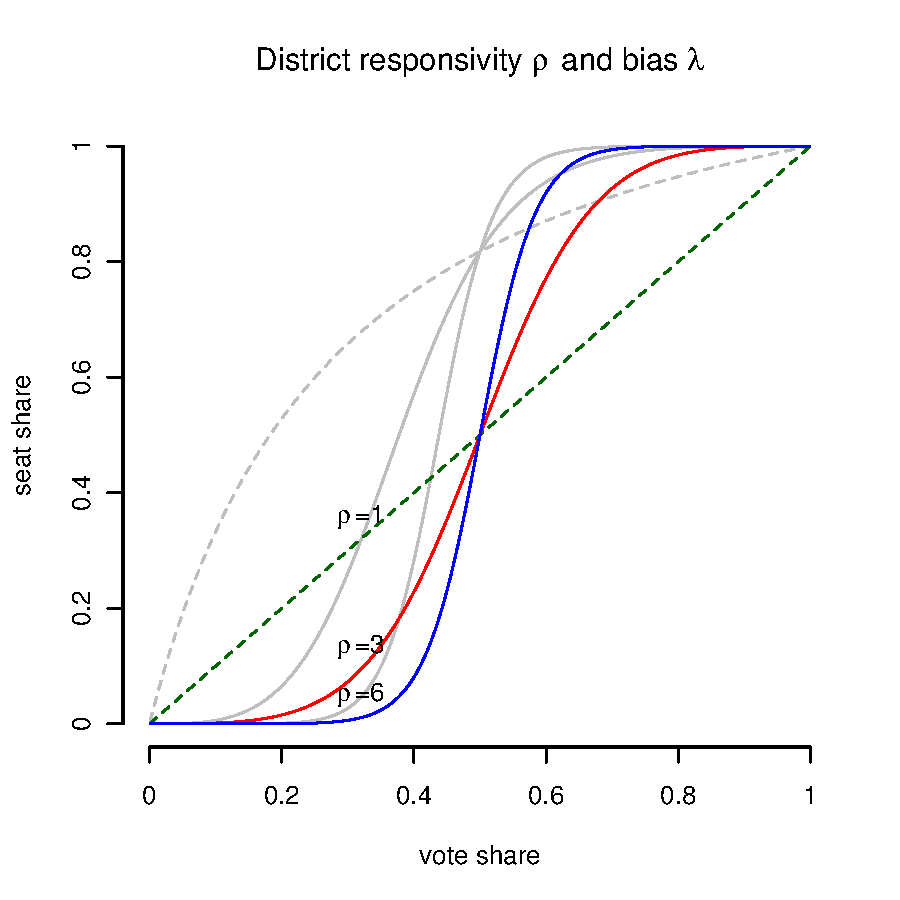
\includegraphics[width=6cm]{../../graphs/rhoLambdaExample.pdf} 
   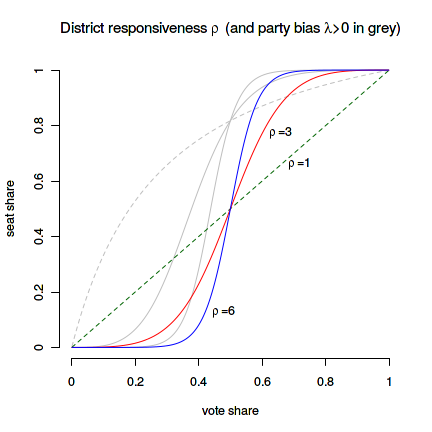
\includegraphics[width=6cm]{../../graphs/rhoExample.png} 
\end{center}

\end{columns}


}
%%%%%%%%%%%%%%%%%%%%%%%%%%%%%%%%%%%%%%%%%%%%%%%%%%%%%%%%%%%%%%%%%%%%%%%%%%%%%%%%%%%%%%%%%%%%
\frame {                      % SLIDE
    \frametitle{Three sources of partisan bias}


\newcommand{\mc}{\multicolumn}
\centering
% %\newcolumntype{d}[1]{D{.}{.}{#1}} % D column with 1 decimal spaces default, usage d{2} for two spaces
%\newcolumntype{d}{D{.}{.}{2}} % D column with space for 2 decimal spaces
%\begin{tabular}{lrdrrrrddrrrrdd}
\resizebox{\textwidth}{!}{
\begin{tabular}{lrrrrrrrrrrrrrr}
          &              &                  &  \mc{3}{c}{Raw votes}      &&  \mc{2}{c}{Vote shares}        && \mc{2}{c}{Seat shares}\\ \cline{4-6} \cline{8-9} \cline{11-12}
%         &  (d)         &    (c/d)         &  a        &  (b)  &  (c)   && \mc{1}{r}{a/c}&   b/c          \\
Districts &  Pop.        &\mc{1}{r}{Turnout}&  left     & right&  total  &&\mc{1}{r}{left}&\mc{1}{r}{right}&&\mc{1}{r}{left}&\mc{1}{r}{right}\\ \hline
\mc{9}{l}{~~\textbf{Gerrymander}}                                                    && &     \\    
1 and 2   &  420         &   .5             &  147      &  63  &  210    &&   .\textbf{7} &   .\textbf{3}  && 1 & 0 \\
3, 4 and 5&  420         &   .5             &  84       &  126 &  210    &&   .\textbf{4} &   .\textbf{6}  && 0 & 1 \\ \hdashline
nationwide&  2100        &   .5             &  546      &  504 &  1050   &&   .52         &   .48          &&.4 &.6 \\ \hline
\mc{9}{l}{~~\textbf{Turnout}}                                                        && &     \\
1 and 2   &  420         &   .\textbf{70}   &  200      &  100 &  300    &&   .67         &   .33          && 1 & 0 \\
3, 4 and 5&  420         &   .\textbf{35}   &  50       &  100 &  150    &&   .33         &   .67          && 0 & 1 \\ \hdashline
nationwide&  2100        &   .5             &  550      &  500 &  1050   &&   .52         &   .48          &&.4 &.6 \\ \hline
\mc{9}{l}{~~\textbf{Malapportionment}}                                               && &     \\ 
1 and 2   & \textbf{600} &   .5             &  200      &  100 &  300    &&   .67         &   .33          && 1 & 0 \\
3, 4 and 5& \textbf{300} &   .5             &  50       &  100 &  150    &&   .33         &   .67          && 0 & 1 \\ \hdashline
nationwide&  2100        &   .5             &  550      &  500 &  1050   &&   .52         &   .48          &&.4 &.6 \\ \hline
\end{tabular}
}

}
%%%%%%%%%%%%%%%%%%%%%%%%%%%%%%%%%%%%%%%%%%%%%%%%%%%%%%%%%%%%%%%%%%%%%%%%%%%%%%%%%%%%%%%%%%%%
\frame {                      % SLIDE
    \frametitle{Obstacle 1: partisan bias breakdown}


Grofman, Koetzle \& Brunell (1997): Three ways to aggregate district returns nationwide

\begin{align}
%v  &= \sum_d v_{d} \times \frac{\text{raw vote}_d}{\text{total raw vote}} \\ % Ri in GKB
%\bar{v}  &= \sum_d v_{d} \times \frac{1}{\text{total districts}} \\% Pi in GKB
%\bar{w}  &= \sum_d v_{d} \times \frac{\text{population}_d}{\text{total population}} % Mi in GKB
v_p  &= \sum_d v_{dp} \times \frac{\text{raw vote}_d}{\text{total raw vote}} \\ % Ri in GKB
\bar{v}_p  &= \sum_d v_{dp} \times \frac{1}{\text{total districts}} \\% Pi in GKB
\bar{w}_p  &= \sum_d v_{dp} \times \frac{\text{population}_d}{\text{total population}} % Mi in GKB
\end{align}

\bigskip \pause

Fitting votes--seats curve with (1), (2), or (3) yields components 

$\rightarrow$ with $v$ you get \textbf{raw} partisan bias

$\rightarrow$ with $\bar{v}$ you get \textbf{gerrymander}-based

$\rightarrow$ with $\bar{w}$ you get \textbf{gerrymander} + \textbf{malapportionment}-based
}
%%%%%%%%%%%%%%%%%%%%%%%%%%%%%%%%%%%%%%%%%%%%%%%%%%%%%%%%%%%%%%%%%%%%%%%%%%%%%%%%%%%%%%%%%%%%
\frame {                      % SLIDE
    \frametitle{Obstacle 1: partisan bias breakdown}

Trick is to estimate $\lambda$ with each national vote measure in turn

\centering

\begin{block}{Formulas:}
\begin{enumerate}
\renewcommand{\theenumi}{\alph{enumi}}
\item raw partisan bias $=\lambda^{v}$
\item gerrymander-based $=\lambda^{\bar{v}}$ 
\item malapportionment-based $=\lambda^{\bar{w}} - \lambda^{\bar{v}}$ 
\item turnout-based $=\lambda^{v} - \lambda^{\bar{w}}$ 
\item a = b + c + d
\end{enumerate}
\end{block}

\bigskip


}
%%%%%%%%%%%%%%%%%%%%%%%%%%%%%%%%%%%%%%%%%%%%%%%%%%%%%%%%%%%%%%%%%%%%%%%%%%%%%%%%%%%%%%%%%%%%
\frame {                      % SLIDE
    \frametitle{Obstacle 2: multi-party competition}

King (1990) is a votes-seats curve for a $P$-party system ($P\geq2$)

\begin{equation*}
 E(s_p) = \frac{e^{\lambda_p} v_p^\rho}{\sum_{q=1}^{P} e^{\lambda_q}  v_q^\rho}
\end{equation*}

\bigskip

\begin{itemize}
\item Akin to switch from dichotomous to multinomial logit regression
\item Restricting $\lambda_1 = 0$ expresses bias relative to party $p=1$ 
\end{itemize}

\pause \bigskip

\alert{In sum:}

Fit equation above using $v$, then $\bar{v}$, then $\bar{w}$; \\ rely on subtraction formulas to get measures of raw partisan bias and its components

}
%%%%%%%%%%%%%%%%%%%%%%%%%%%%%%%%%%%%%%%%%%%%%%%%%%%%%%%%%%%%%%%%%%%%%%%%%%%%%%%%%%%%%%%%%%%%
\section{Mexican C\'amara de Diputados elections}
%%%%%%%%%%%%%%%%%%%%%%%%%%%%%%%%%%%%%%%%%%%%%%%%%%%%%%%%%%%%%%%%%%%%%%%%%%%%%%%%%%%%%%%%%%%%
\frame {
    \frametitle{Background on Mexico}

\begin{itemize}

%\item 32 states, 2.5k municipalities, 67k electoral \emph{secciones}

\item Hegemonic party 1929--1997 

\item Three major parties: \begin{tabular}{ccc} PRD & PRI & PAN \\ left & & right \end{tabular} and minors

\item Lower chamber of Congress elected every 3 years, \\ concurrent w presidential race every 6 years

\item Mixed system: 300 SMD + 200 PR seats

\item Single-term limits removed in 2018

\item Independent board (IFE) manages elections and redistricting

\end{itemize}
}
%%%%%%%%%%%%%%%%%%%%%%%%%%%%%%%%%%%%%%%%%%%%%%%%%%%%%%%%%%%%%%%%%%%%%%%%%%%%%%%%%%%%%%%%%%%%
\frame {                      % SLIDE
    \frametitle{Obstacle 3: small-N}

\begin{itemize}
\item A general election with $P$ parties offers $P$ data points to fit a votes-seats curve
\item $P$ typically small
\item Multi-year approach: pool historic record... may compare apples/oranges in long-haul
\item Single-election approach preferable... but requires data multiplication strategy 
\end{itemize}
}
%%%%%%%%%%%%%%%%%%%%%%%%%%%%%%%%%%%%%%%%%%%%%%%%%%%%%%%%%%%%%%%%%%%%%%%%%%%%%%%%%%%%%%%%%%%%
\frame {                      % SLIDE
    \frametitle{Monte Carlo simulation}
\begin{itemize}
\item Linzer (2012): approximates prob.\ distribution of national party vote returns from observed district outcomes (FMM)
\item Use to simulate 1,000 elections
\end{itemize}

\begin{center}
\begin{tabular}{cc}
   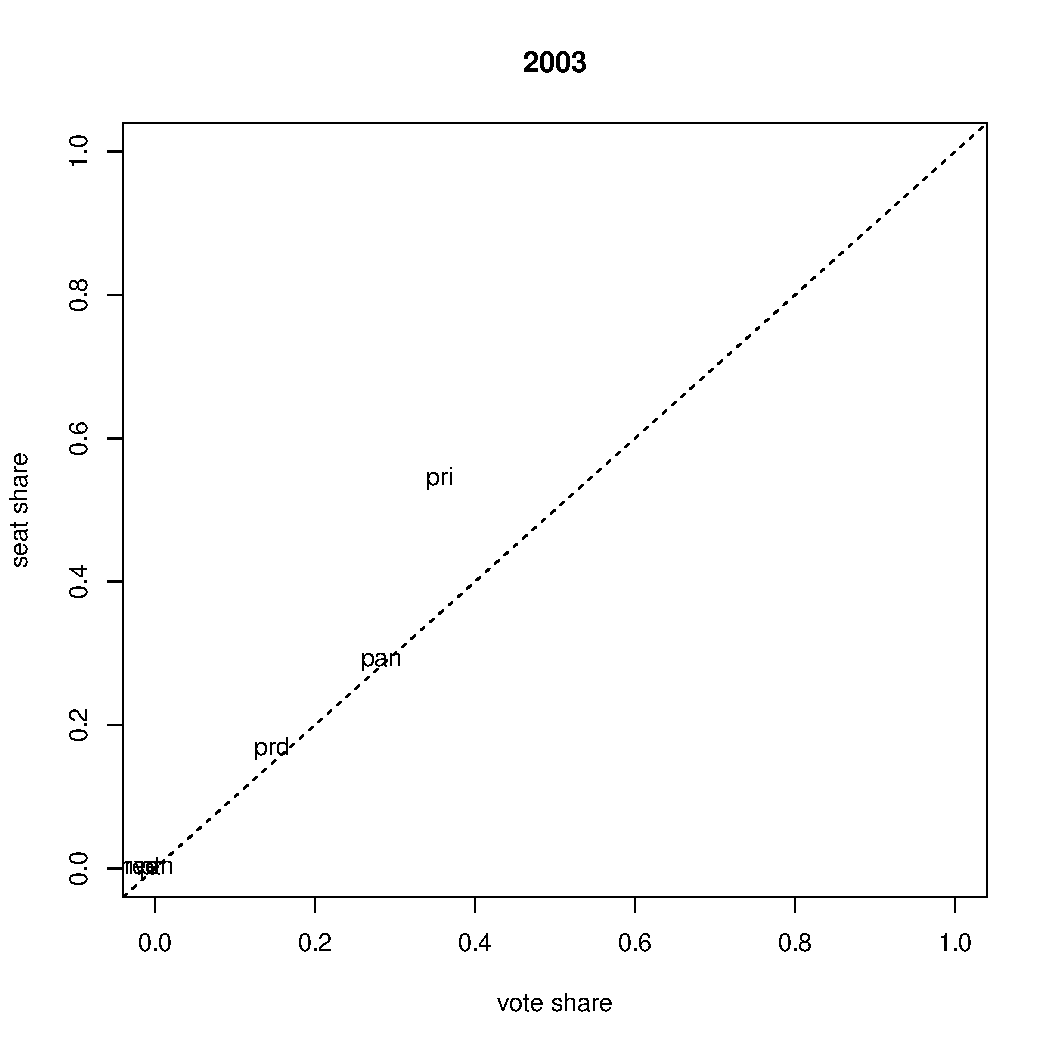
\includegraphics[width=.3\textwidth]{../../graphs/vsNosims2003.pdf} &
   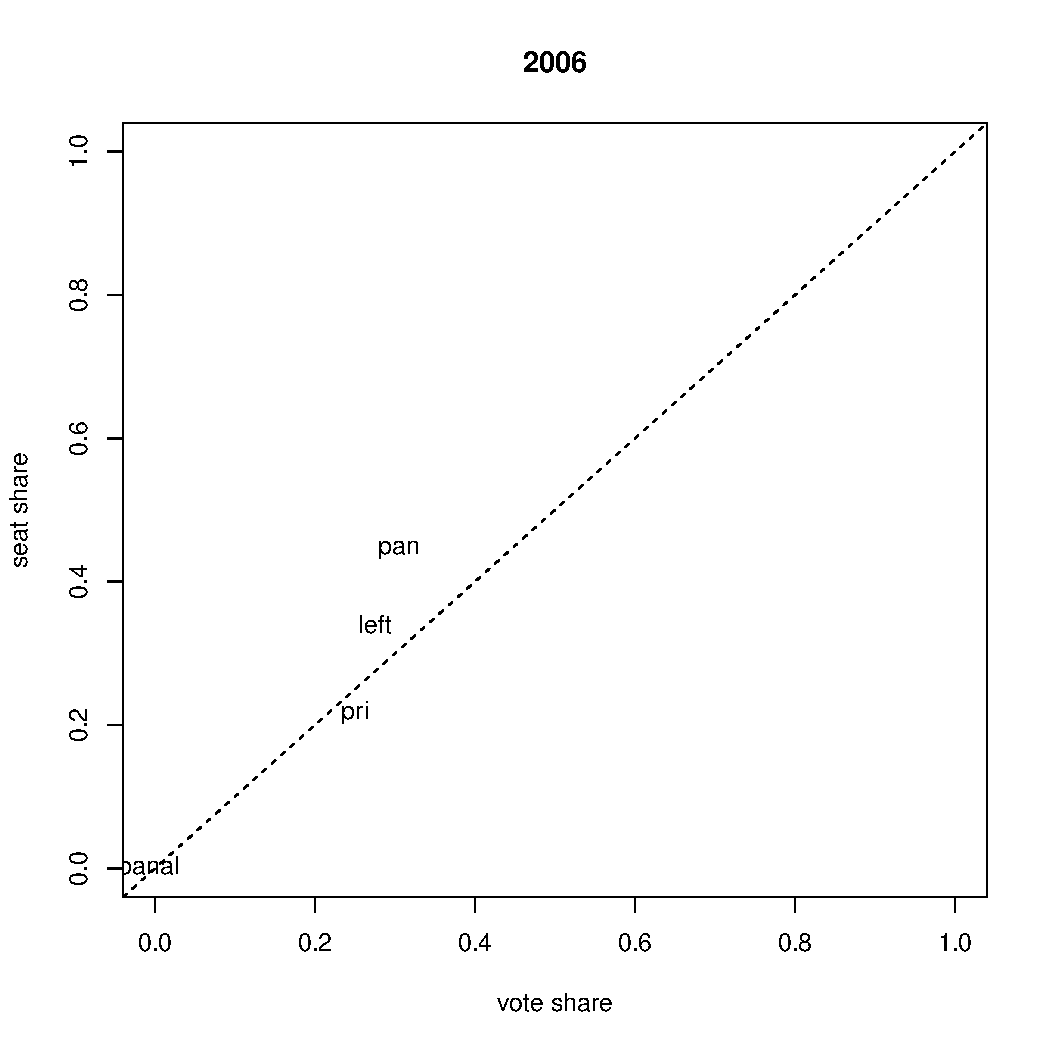
\includegraphics[width=.3\textwidth]{../../graphs/vsNosims2006.pdf} \\
   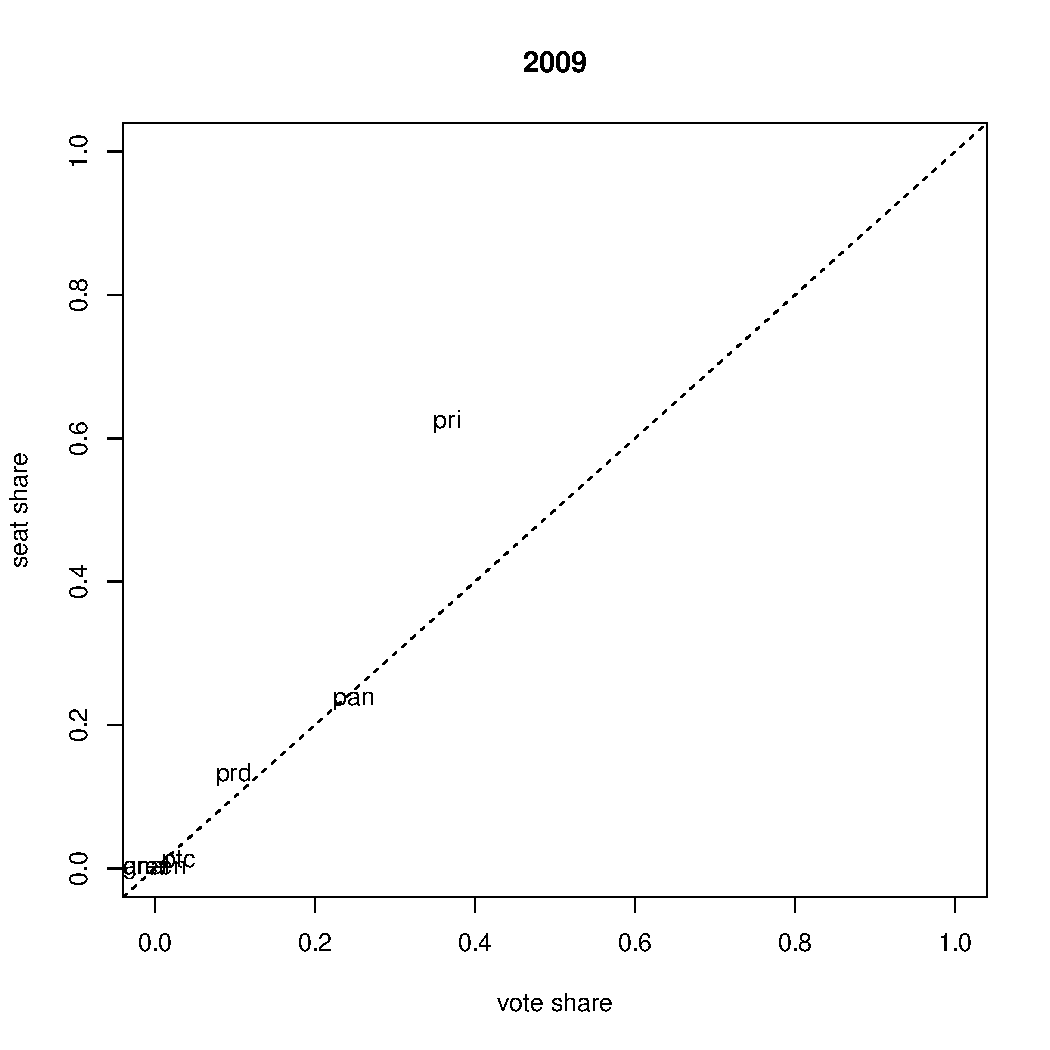
\includegraphics[width=.3\textwidth]{../../graphs/vsNosims2009.pdf} &
   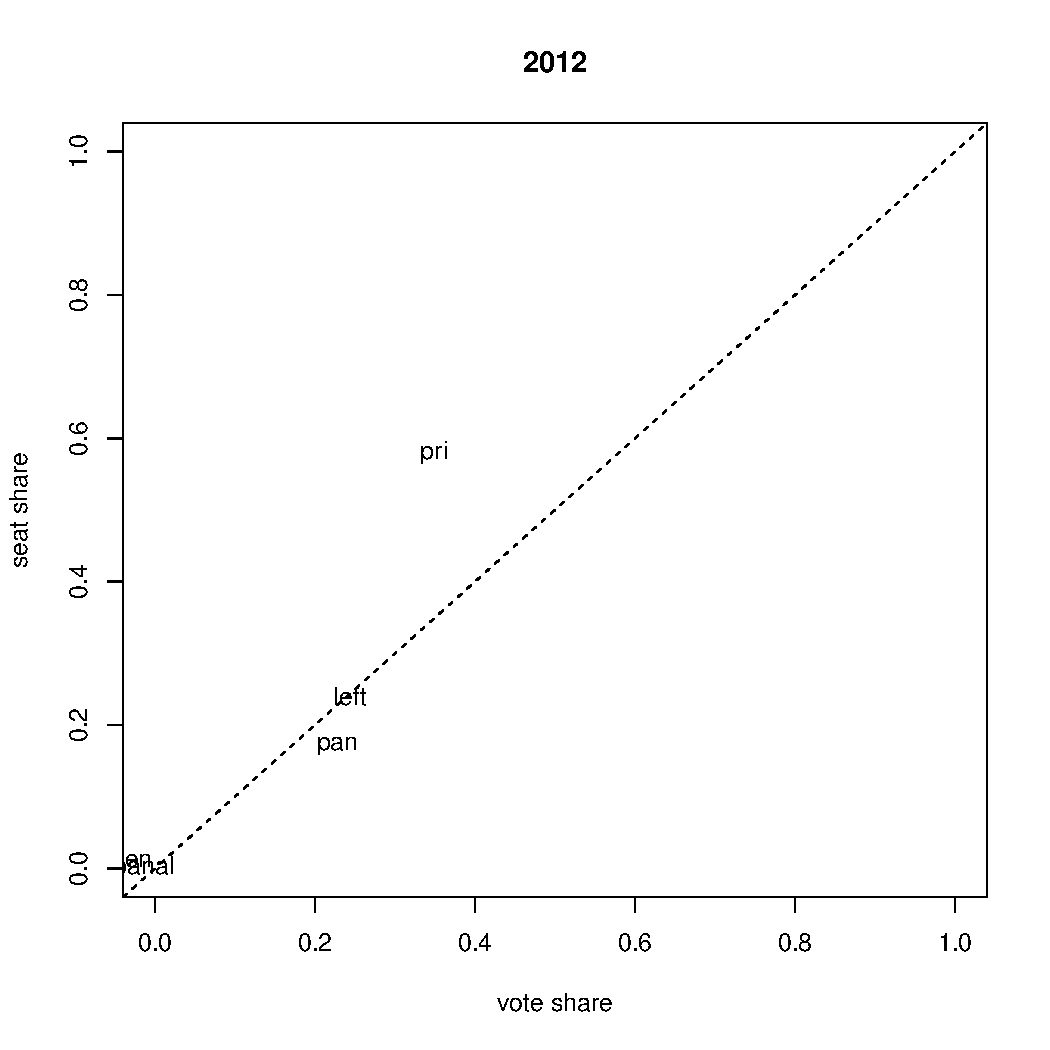
\includegraphics[width=.3\textwidth]{../../graphs/vsNosims2012.pdf} \\
\end{tabular}
\end{center}
}
%%%%%%%%%%%%%%%%%%%%%%%%%%%%%%%%%%%%%%%%%%%%%%%%%%%%%%%%%%%%%%%%%%%%%%%%%%%%%%%%%%%%%%%%%%%%
\frame {                      % SLIDE
    \frametitle{Monte Carlo simulation}
\begin{itemize}
\item Linzer (2012): approximates prob.\ distribution of national party vote returns from observed district outcomes (FMM)
\item Use to simulate 1,000 elections
\end{itemize}

\begin{center}
\begin{tabular}{cc}
   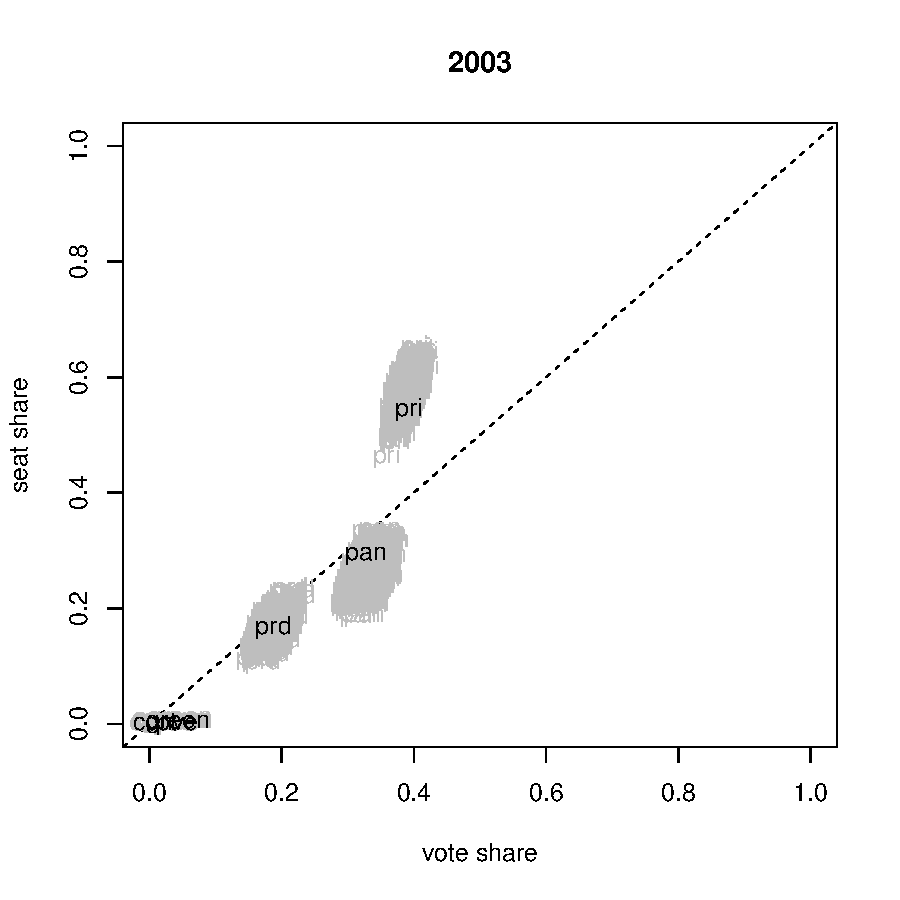
\includegraphics[width=.3\textwidth]{../../graphs/vs2003.pdf} &
   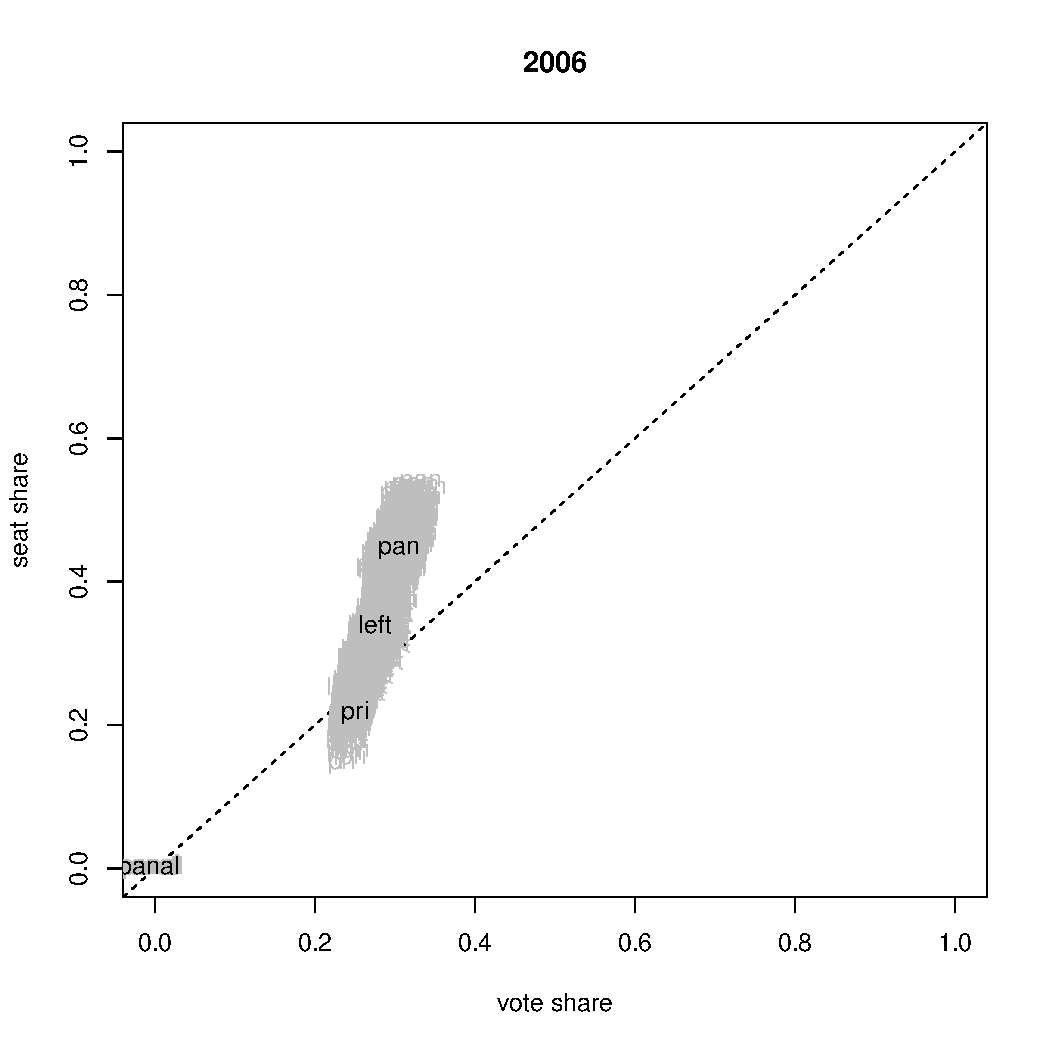
\includegraphics[width=.3\textwidth]{../../graphs/vs2006.pdf} \\
   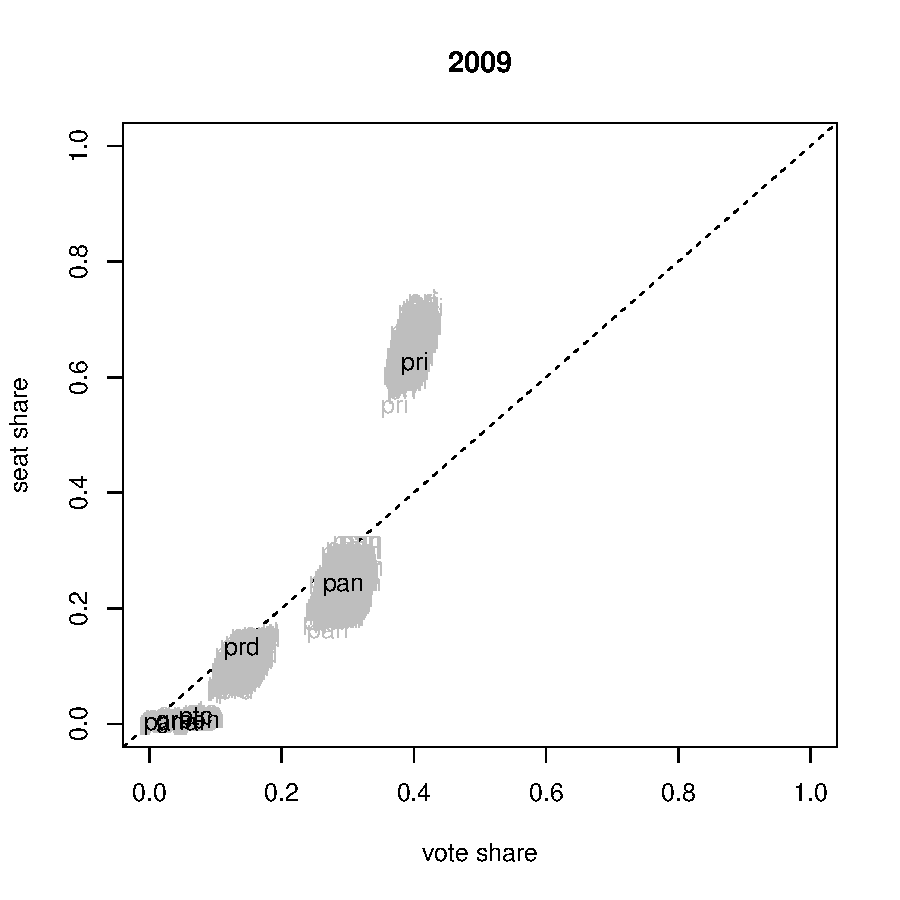
\includegraphics[width=.3\textwidth]{../../graphs/vs2009.pdf} &
   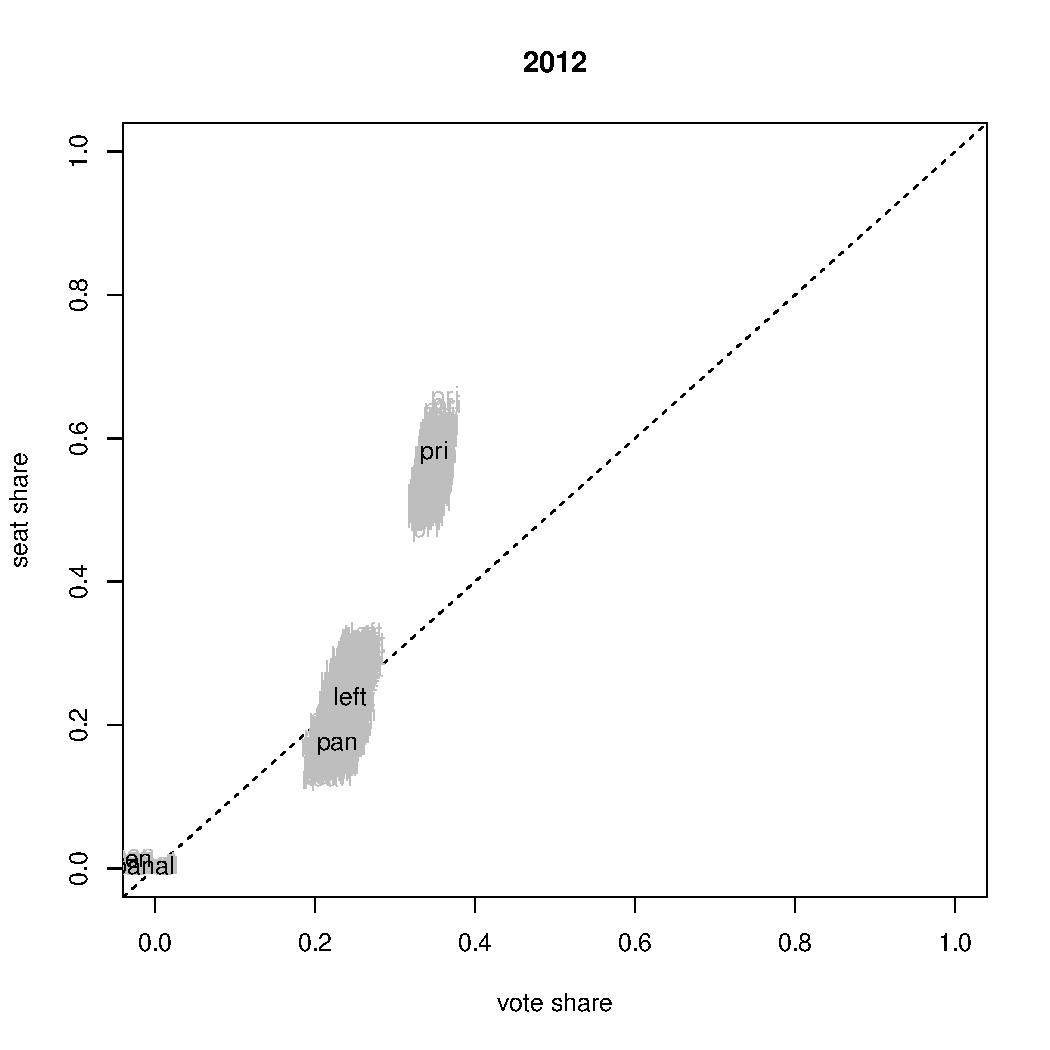
\includegraphics[width=.3\textwidth]{../../graphs/vs2012.pdf} \\
\end{tabular}
\end{center}
}
% %%%%%%%%%%%%%%%%%%%%%%%%%%%%%%%%%%%%%%%%%%%%%%%%%%%%%%%%%%%%%%%%%%%%%%%%%%%%%%%%%%%%%%%%%%%% 
% \frame{                      % SLIDE
%     \frametitle{Two components 2009}

% \begin{center}
% 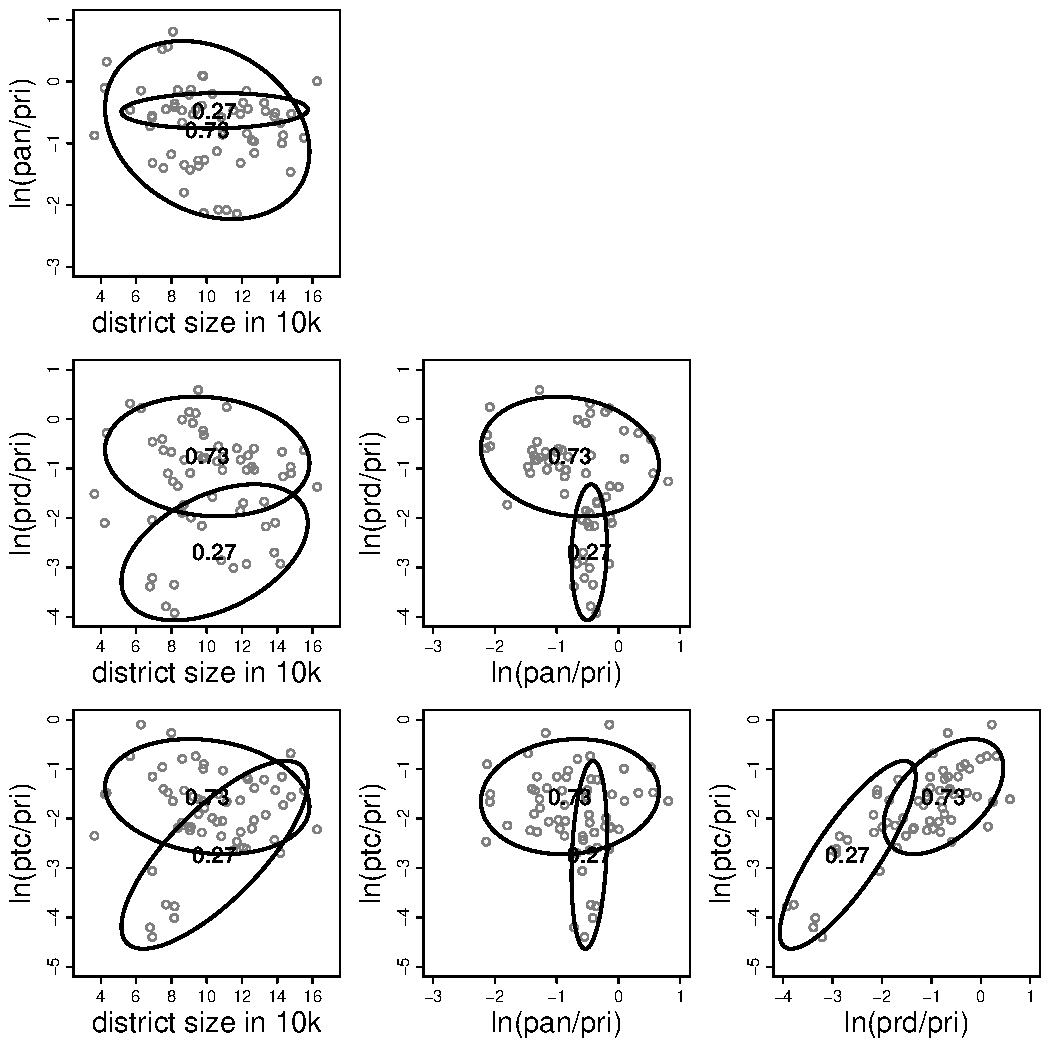
\includegraphics[width=.75\textwidth]{../../graphs/linzerLogVot2009-1.pdf} 
% \end{center}
% }
%%%%%%%%%%%%%%%%%%%%%%%%%%%%%%%%%%%%%%%%%%%%%%%%%%%%%%%%%%%%%%%%%%%%%%%%%%%%%%%%%%%%%%%%%%%%%%%%
\frame {                      % SLIDE
    \frametitle{Mixture model}
\begin{itemize}
\item Combines the properties of two or more prob.\ density functions: can approximate any arbitrary distribution
\item Seek components (multivariate normals)  and weights of log-ratio votes shares
\end{itemize}

\centering

   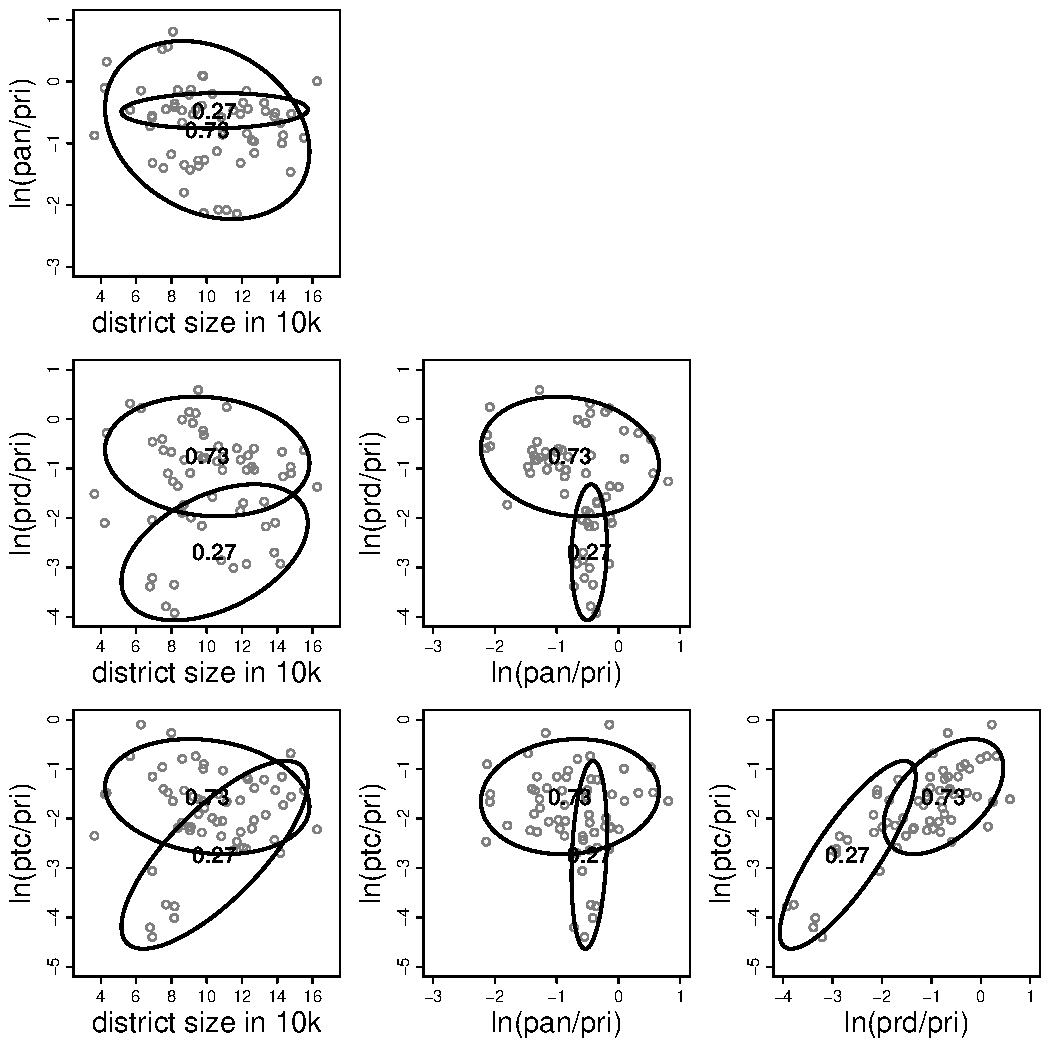
\includegraphics[width=6cm]{../../graphs/linzerLogVot2009-1.pdf} 
 
}
%%%%%%%%%%%%%%%%%%%%%%%%%%%%%%%%%%%%%%%%%%%%%%%%%%%%%%%%%%%%%%%%%%%%%%%%%%%%%%%%%%%%%%%%%%%% 
\section{Malapportionment}
%%%%%%%%%%%%%%%%%%%%%%%%%%%%%%%%%%%%%%%%%%%%%%%%%%%%%%%%%%%%%%%%%%%%%%%%%%%%%%%%%%%%%%%%%%%% 
\frame{                      % SLIDE
    \frametitle{One Mexican--one vote?}

Malapportionment occurs when sparsely populated areas get the same representation as the densely populated

\bigskip

Can arise by commission or by omission (or by accident)

\bigskip

Census lag: most recent decennial census must be used 

\begin{itemize}
\item ... but no obligation to redistrict as soon as available
\item 6-year lag on average: 199\textbf{7}, 200\textbf{6}, 201\textbf{5}
\item 2015 map abandoned
\item board considers $\pm15\%$ imbalance normal (!)
\end{itemize}


}
%%%%%%%%%%%%%%%%%%%%%%%%%%%%%%%%%%%%%%%%%%%%%%%%%%%%%%%%%%%%%%%%%%%%%%%%%%%%%%%%%%%%%%%%%%%% 
\frame{                      % SLIDE
    \frametitle{District populations: linear projection}

\centering

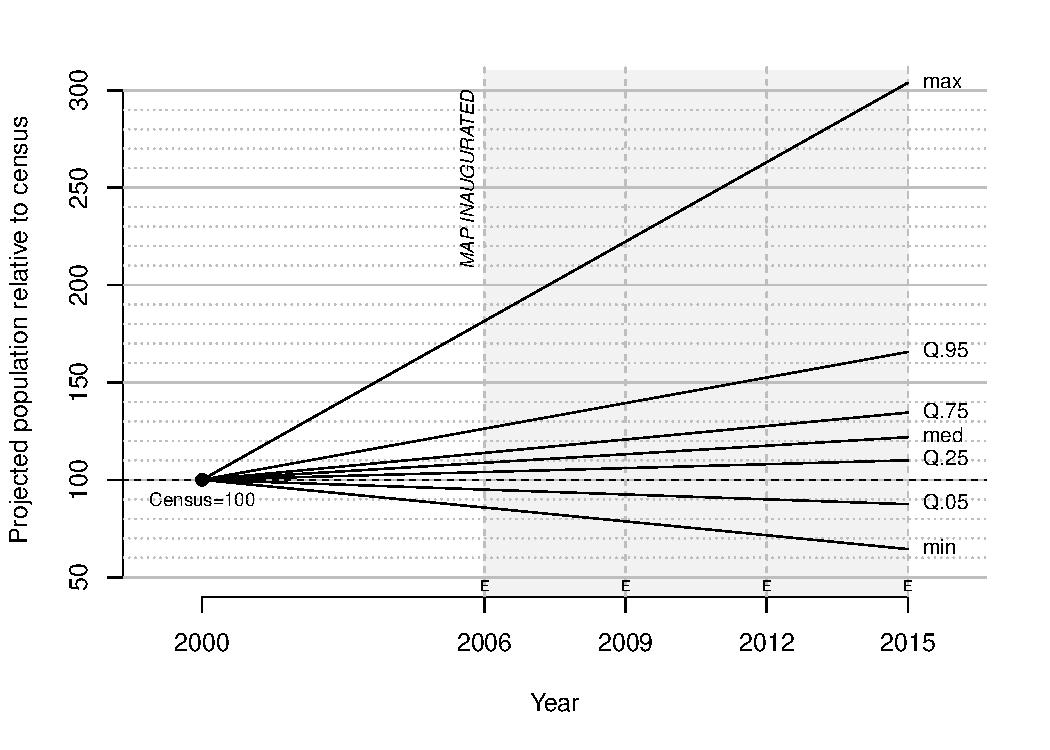
\includegraphics[width=.99\textwidth]{../../graphs/disRelPopProj2006map.pdf}

%\pause

Plus: bureaucratic leeway in new district sizes %$\rightarrow$ substantial malapportionment


}
%%%%%%%%%%%%%%%%%%%%%%%%%%%%%%%%%%%%%%%%%%%%%%%%%%%%%%%%%%%%%%%%%%%%%%%%%%%%%%%%%%%%%%%%%%%% 
\frame{                      % SLIDE
    \frametitle{Malapportionment is substantial}

\centering

%$RRI = \frac{1/\text{district size}}{300/\text{national population}} = \frac{Q}{\text{district size}}$
$RRI = \frac{nat. pop./300}{\text{district size}}$

\bigskip

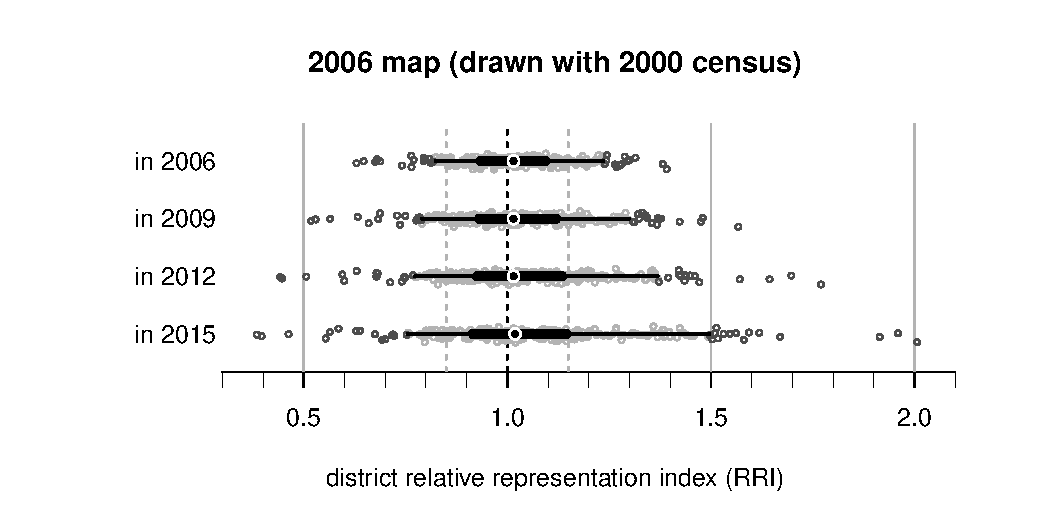
\includegraphics[width=.6\textwidth]{../../graphs/rrin0615d0.pdf} \\
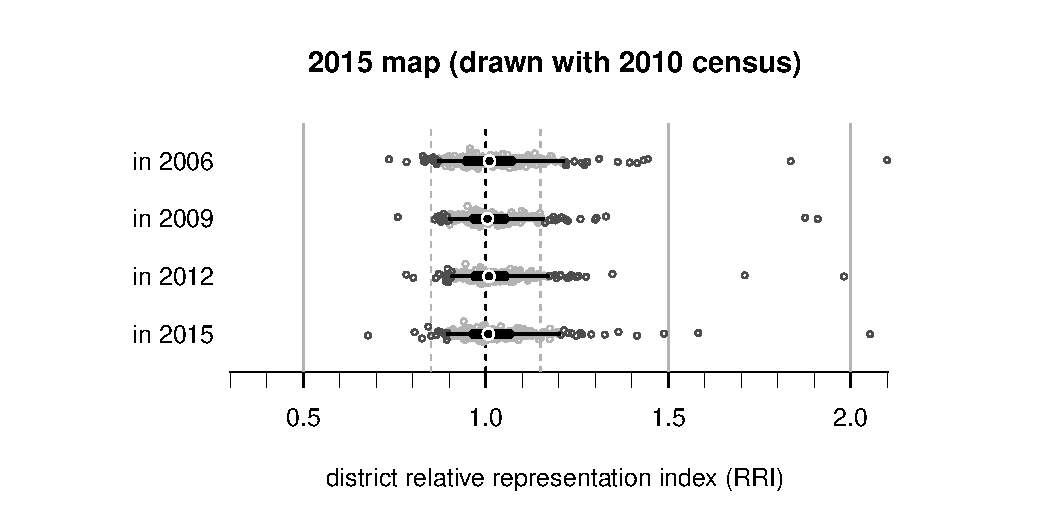
\includegraphics[width=.6\textwidth]{../../graphs/rrin0615d3.pdf} 


}
%%%%%%%%%%%%%%%%%%%%%%%%%%%%%%%%%%%%%%%%%%%%%%%%%%%%%%%%%%%%%%%%%%%%%%%%%%%%%%%%%%%%%%%%%%%% 
\section{Results}
%%%%%%%%%%%%%%%%%%%%%%%%%%%%%%%%%%%%%%%%%%%%%%%%%%%%%%%%%%%%%%%%%%%%%%%%%%%%%%%%%%%%%%%%%%%% 
\frame{                      % SLIDE
    \frametitle{Estimation}

Votes--seats curve fitted with MCMC (\texttt{Jags} via \texttt{R})

\bigskip

100k iterations of 3 chains, every 500th obs.\ of last 50k used to sample posterior density

\bigskip

Visual inspection of model parameters to verify chain convergence

}
%%%%%%%%%%%%%%%%%%%%%%%%%%%%%%%%%%%%%%%%%%%%%%%%%%%%%%%%%%%%%%%%%%%%%%%%%%%%%%%%%%%%%%%%%%%% 
\frame{                      % SLIDE
    \frametitle{Results: raw partisan bias}

\centering
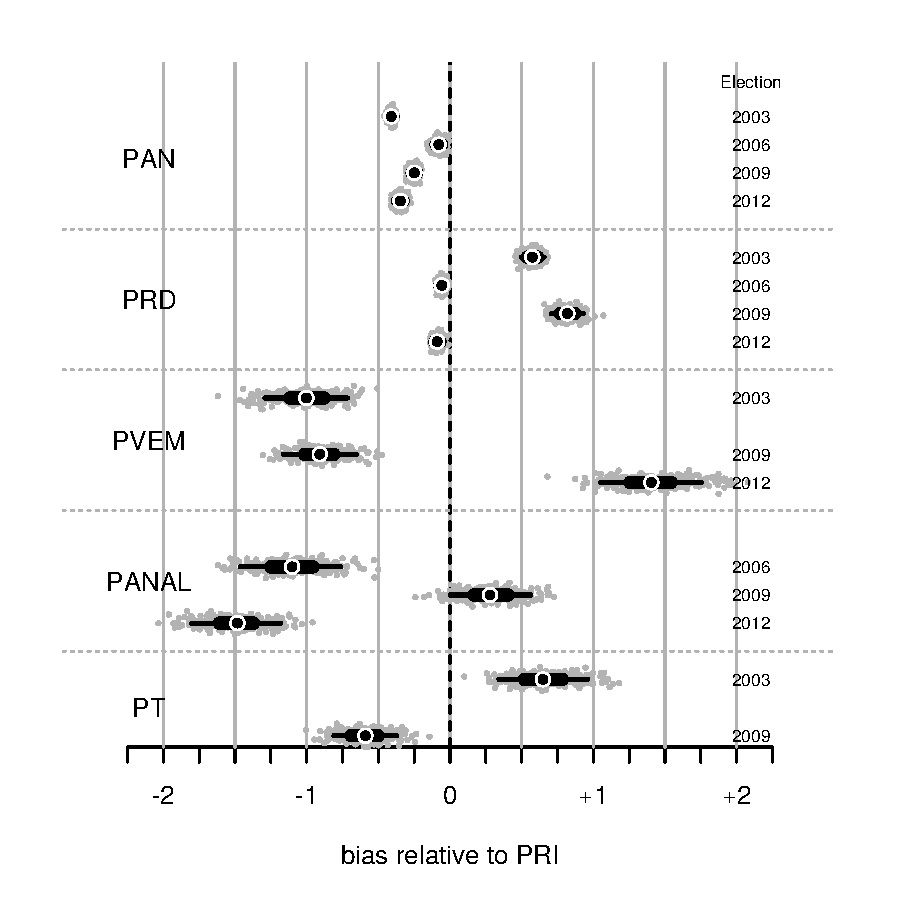
\includegraphics[width=.8\textwidth]{../../graphs/bias200612d0R.pdf} 

}
%%%%%%%%%%%%%%%%%%%%%%%%%%%%%%%%%%%%%%%%%%%%%%%%%%%%%%%%%%%%%%%%%%%%%%%%%%%%%%%%%%%%%%%%%%%% 
\frame{                      % SLIDE
    \frametitle{Results: components}

 \begin{columns}[c]

\column{.65\textwidth}

\newcommand{\mc}{\multicolumn}
\setbeamerfont{alerted text}{series=\bfseries} % makes alert boldface
%\newcolumntype{d}[1]{D{.}{.}{#1}} % D column with 1 decimal spaces default, usage d{2} for two spaces
%\newcolumntype{d}{D{.}{.}{2}} % D column with space for 2 decimal spaces
\resizebox{.95\textwidth}{!}{
\centering
\begin{tabular}{lrrr|rrr}
              &  \mc{3}{c|}{Actual map} & \mc{3}{c}{Hypothetical map} \\
partisan bias &  \mc{1}{c}{\textsc{pan}--\textsc{pri}}  &  \mc{1}{c}{\textsc{prd}--\textsc{pri}} &  \mc{1}{c|}{min--\textsc{pri}}  & \mc{1}{c}{\textsc{pan}--\textsc{pri}}  &  \mc{1}{c}{\textsc{prd}--\textsc{pri}} &  \mc{1}{c}{min--\textsc{pri}} \\  \hline
\mc{4}{l}{\textbf{~2003 election}}     & \mc{3}{c}{(with 2006 map)} \\
raw           & $-$.37 &  +.72 &$-$1.01 &  $-$.41 &  +.57 &$-$1.00   \\ [-1ex]
              &   \mc{1}{r}{\footnotesize{(0)}}  &   \mc{1}{r}{\footnotesize{(0)}} &  \mc{1}{r|}{\footnotesize{(0)}}  &  \mc{1}{r}{\footnotesize{(0)}}  &   \mc{1}{r}{\footnotesize{(0)}} &  \mc{1}{r}{\footnotesize{(0)}}    \\
gerrym.       & $-$.09 &  +.69 &$-$.88 &  $-$.13 &  +.62 &$-$.90   \\ [-1ex]
              &   \mc{1}{r}{\footnotesize{(0)}}  &   \mc{1}{r}{\footnotesize{(0)}} &  \mc{1}{r|}{\footnotesize{(0)}}  &  \mc{1}{r}{\footnotesize{(0)}}  &   \mc{1}{r}{\footnotesize{(0)}} &  \mc{1}{r}{\footnotesize{(0)}}    \\
turnout       & \alert<2>{$-$.26} &\alert<2,5>{$-$.11} &\alert<2>{$-$.08} &  \alert<2>{$-$.26} &\alert<2>{$-$.09} &\alert<2>{$-$.09}   \\ [-1ex]
              &   \mc{1}{r}{\footnotesize{(0)}}  &   \mc{1}{r}{\footnotesize{(0)}} &  \mc{1}{r|}{\footnotesize{(0)}}  &  \mc{1}{r}{\footnotesize{(0)}}  &   \mc{1}{r}{\footnotesize{(0)}} &  \mc{1}{r}{\footnotesize{(0)}}    \\
malapp.       & $-$.01 &  \alert<3,5>{+.14} &$-$.05 &  \alert<4>{$-$.02} &  \alert<4>{+.05} &\alert<4>{$-$.02}   \\ [-1ex]
              &   \mc{1}{r}{\footnotesize{(.11)}}  &   \mc{1}{r}{\footnotesize{(0)}} &  \mc{1}{r|}{\footnotesize{(0)}}  &  \mc{1}{r}{\footnotesize{(.12)}} &   \mc{1}{r}{\footnotesize{(0)}} &  \mc{1}{r}{\footnotesize{(0)}}    \\
\mc{7}{l}{\textbf{~2006 election}}                                 \\
raw           & $-$.08 &$-$.06 & -1.10  &        &        &        \\ [-1ex]
              &   \mc{1}{r}{\footnotesize{(0)}}  &   \mc{1}{r}{\footnotesize{(0)}} &  \mc{1}{r|}{\footnotesize{(0)}}  & & & \\
gerrym.       &   \alert<5>{+.28} &  \alert<5>{+.30} &$-$.62  &        &        &        \\ [-1ex]
              &   \mc{1}{r}{\footnotesize{(0)}}  &   \mc{1}{r}{\footnotesize{(0)}} &  \mc{1}{r|}{\footnotesize{(0)}}  & & & \\
turnout       & \alert<2,5>{$-$.36} &\alert<2,5>{$-$.41} &\alert<2>{$-$.43}  &        &        &        \\ [-1ex]
              &   \mc{1}{r}{\footnotesize{(0)}}  &   \mc{1}{r}{\footnotesize{(0)}} &  \mc{1}{r|}{\footnotesize{(0)}}  & & & \\
malapp.       & $-$.00 &  \alert<3>{+.05} &$-$.05  &        &        &        \\ [-1ex]
              &   \mc{1}{r}{\footnotesize{(.42)}}  &   \mc{1}{r}{\footnotesize{(0)}} &  \mc{1}{r|}{\footnotesize{(0)}}  & & & \\
\mc{7}{l}{\textbf{~2009 election}}                                 \\ 
raw           & $-$.25 &  +.82 &$-$.91  &        &        &        \\  [-1ex]
              &   \mc{1}{r}{\footnotesize{(0)}}  &   \mc{1}{r}{\footnotesize{(0)}} &  \mc{1}{r|}{\footnotesize{(0)}}  & & & \\
gerrym.       & $-$.11 & \alert<5>{+1.01} &$-$.79  &        &        &        \\  [-1ex]
              &   \mc{1}{r}{\footnotesize{(0)}}  &   \mc{1}{r}{\footnotesize{(0)}} &  \mc{1}{r|}{\footnotesize{(0)}}  & & & \\
turnout       & \alert<2>{$-$.14} &\alert<2,5>{$-$.24} &\alert<2>{$-$.12}  &        &        &        \\  [-1ex]
              &   \mc{1}{r}{\footnotesize{(0)}}  &   \mc{1}{r}{\footnotesize{(0)}} &  \mc{1}{r|}{\footnotesize{(0)}}  & & & \\
malapp.       & $-$.00 &  \alert<3>{+.05} &$-$.00  &        &        &        \\  [-1ex]
              &   \mc{1}{r}{\footnotesize{(.36)}}  &   \mc{1}{r}{\footnotesize{(0)}} &  \mc{1}{r|}{\footnotesize{(0)}}  & & & \\
\mc{4}{l}{\textbf{~2012 election}}      & \mc{3}{c}{(with 2015 map)} \\
raw           & $-$.35 &$-$.09 & +1.40  &  $-$.32 &$-$.13 & +1.03  \\  [-1ex]
              &   \mc{1}{r}{\footnotesize{(0)}}  &   \mc{1}{r}{\footnotesize{(0)}} &  \mc{1}{r|}{\footnotesize{(0)}}  &  \mc{1}{r}{\footnotesize{(0)}}  &   \mc{1}{r}{\footnotesize{(0)}} &  \mc{1}{r}{\footnotesize{(0)}}    \\
gerrym.       & $-$.28 &$-$.07 & +1.41  &  $-$.24 &$-$.05 & +1.02  \\  [-1ex]
              &   \mc{1}{r}{\footnotesize{(0)}}  &   \mc{1}{r}{\footnotesize{(0)}} &  \mc{1}{r|}{\footnotesize{(0)}}  &  \mc{1}{r}{\footnotesize{(0)}}  &   \mc{1}{r}{\footnotesize{(.06)}} &  \mc{1}{r}{\footnotesize{(0)}}    \\
turnout       & \alert<2>{$-$.07} &\alert<2>{$-$.08} &  +.02  &  \alert<2>{$-$.08} &\alert<2>{$-$.09} &  +.01  \\  [-1ex]
              &   \mc{1}{r}{\footnotesize{(.02)}}  &   \mc{1}{r}{\footnotesize{(0)}} &  \mc{1}{r|}{\footnotesize{(0)}}  &  \mc{1}{r}{\footnotesize{(.26)}}  &   \mc{1}{r}{\footnotesize{(0)}} &  \mc{1}{r}{\footnotesize{(0)}}    \\
malapp.       &   +.01 &  \alert<3>{+.06} &$-$.02  &  \alert<4>{$-$.00} &  \alert<4>{+.01} &  \alert<4>{+.00}  \\  [-1ex]
              &   \mc{1}{r}{\footnotesize{(.42)}} &   \mc{1}{r}{\footnotesize{(0)}} &  \mc{1}{r|}{\footnotesize{(0)}}  &  \mc{1}{r}{\footnotesize{(.38)}}  &   \mc{1}{r}{\footnotesize{(0)}} &  \mc{1}{r}{\footnotesize{(0)}}    \\ \hline 
\end{tabular}
}

\column{.35\textwidth}

\begin{itemize}
\item<2-> Turnout always pro-PRI
\item<3-> Malapp.\ always pro-left
\item<4-> Redistricting abates malapp. 
\item<5-> Possibly cancelling effects 
\end{itemize}

\end{columns}

}
% %%%%%%%%%%%%%%%%%%%%%%%%%%%%%%%%%%%%%%%%%%%%%%%%%%%%%%%%%%%%%%%%%%%%%%%%%%%%%%%%%%%%%%%%%%%%%%%%
% \frame {                      % SLIDE
%     \frametitle{Use swing ratios to compare two maps}

% \begin{enumerate}
% \item Simulate 5k 2009 elections with status quo map for each party
% \item Repeat using abandoned map
% \item Pool simulations together and regress
% \item Coefficient $\beta_3$ measures and tests change in \\ party's swing ratio \emph{due to redistricting} 
% \end{enumerate}

% \bigskip

% $s = \beta_0 + \beta_1 v + \beta_2 dis2015 + \beta_3 v \times dis2015 + \texttt{error}$

% }
% %%%%%%%%%%%%%%%%%%%%%%%%%%%%%%%%%%%%%%%%%%%%%%%%%%%%%%%%%%%%%%%%%%%%%%%%%%%%%%%%%%%%%%%%%%%%%%%%
% \frame {                      % SLIDE
%     \frametitle{Results}
% \begin{center}

% % \begin{tabular}{lrrrrrr}
% %                    & \multicolumn{2}{c}{PAN}   & \multicolumn{2}{c}{PRI}   & \multicolumn{2}{c}{Left}   \\
% %                    & $\hat{\beta}$ & $p$-val. & $\hat{\beta}$ & $p$-val. & $\hat{\beta}$ & $p$-val.  \\ \hline
% % ~~\textbf{2006 election} \\
% % $V$                &     1.94 & $<.001$&   2.27 &$<.001$&   1.91 &$<.001$\\
% % $V \times$ dis2015 &     \alert<2>{+.45} & $<.001$&  $-.01$&  .809 &  $-.04$&  .183 \\
% % ~~\textbf{2009 election} \\
% % $V$                &     1.95 & $<.001$&   2.27 &$<.001$&   1.67 &$<.001$\\
% % $V \times$ dis2015 &    $-.13$&   .003 &   +.04 &  .354 &  $-.02$&  .623 \\
% % ~~\textbf{2012 election} \\
% % $V$                &     2.24 &$<.001$ &   3.99 &$<.001$&   2.39 &$<.001$\\
% % $V \times$ dis2015 &     +.02 &   .604 &   +.03 &  .720 &  $-.06$&  .103 \\ \hline
% % \end{tabular}

% \begin{tabular}{lr@{}lr@{}lr@{}l}
%                    & \multicolumn{2}{c}{PAN}   & \multicolumn{2}{c}{PRI}   & \multicolumn{2}{c}{Left} \\ \hline
% ~~\textbf{2006 election} \\
% $v$                &     1.94 & $^{***}$&   2.27 & $^{***}$&   1.91 & $^{***}$\\
% $v \times$ dis2015 &     \alert{+.45} & $^{***}$&  $-.01$&        &  $-.04$&        \\
% ~~\textbf{2009 election} \\
% $v$                &     1.95 & $^{***}$&   2.27 & $^{***}$&   1.67 & $^{***}$\\
% $v \times$ dis2015 &    \alert{$-.13$}& $^{***}$&   +.04 &        &  $-.02$&        \\
% ~~\textbf{2012 election} \\
% $v$                &     2.24 & $^{***}$&   3.99 & $^{***}$&   2.39 & $^{***}$\\
% $v \times$ dis2015 &     +.02 &        &   +.03 &       &  \alert{$-.06$} &  $^{*}$ \\ \hline
% \multicolumn{7}{l}{\footnotesize{$^{***} <.01$, $^{*} <.1$}}
% \end{tabular}

% \end{center}
% }
%%%%%%%%%%%%%%%%%%%%%%%%%%%%%%%%%%%%%%%%%%%%%%%%%%%%%%%%%%%%%%%%%%%%%%%%%%%%%%%%%%%%%%%%%%%%%%%%
\section{Final remarks}
%%%%%%%%%%%%%%%%%%%%%%%%%%%%%%%%%%%%%%%%%%%%%%%%%%%%%%%%%%%%%%%%%%%%%%%%%%%%%%%%%%%%%%%%%%%% 
\begin{frame}\label{fr:MxMapProj}                      % SLIDE

    \frametitle{The bigger project}

\emph{Draw Mexico} project = offspring of \emph{Public Mapping Project in U.S.}

\bigskip

Remove opaqueness from redistricting process 

\bigskip

\texttt{DistrictBuilder} is open-source, web-based software %({\footnotesize \url{www.districtbuilder.org}}):

\begin{itemize}

\item enables widespread DIY redistricting thru cloud computing

\item  internet lets anyone draw/inspect maps: crowdsourcing

\item redistricting contests in 6 US states $\rightarrow$ hundreds of legal plans

\end{itemize}

\bigskip

Application to \alert{Mexico} \href{http://23.21.151.172/}{\beamergotobutton{Link: MexDemo}} (Donations anyone?) 

\end{frame}
%%%%%%%%%%%%%%%%%%%%%%%%%%%%%%%%%%%%%%%%%%%%%%%%%%%%%%%%%%%%%%%%%%%%%%%%%%%%%%%%%%%%%%%%%%%%%%%%
\frame {                      % SLIDE
    \frametitle{Findings \& next steps}

\begin{enumerate}

\item Rel.\ to the right, persistent pro-PRI, and esp.\ pro-left raw bias 

\item Malapportionent effects are (surprisingly) small

\item Pro-PRI turnout-based bias  

\item Gerrymander effects large and volatile

\item District lines can compensate for turnout disadvantage

\item To-do: add PR-tier to analysis

\item To-do: inspect inter-election volatility

\end{enumerate}

\pause

\bigskip

\center{\textbf{\Large{Thank you!}}}

}
%%%%%%%%%%%%%%%%%%%%%%%%%%%%%%%%%%%%%%%%%%%%%%%%%%%%%%%%%%%%%%%%%%%%%%%%%%%%%%%%%%%%%%%%%%%% 
\frame{                      % SLIDE
    \frametitle{The redistricting process}
\begin{center}
   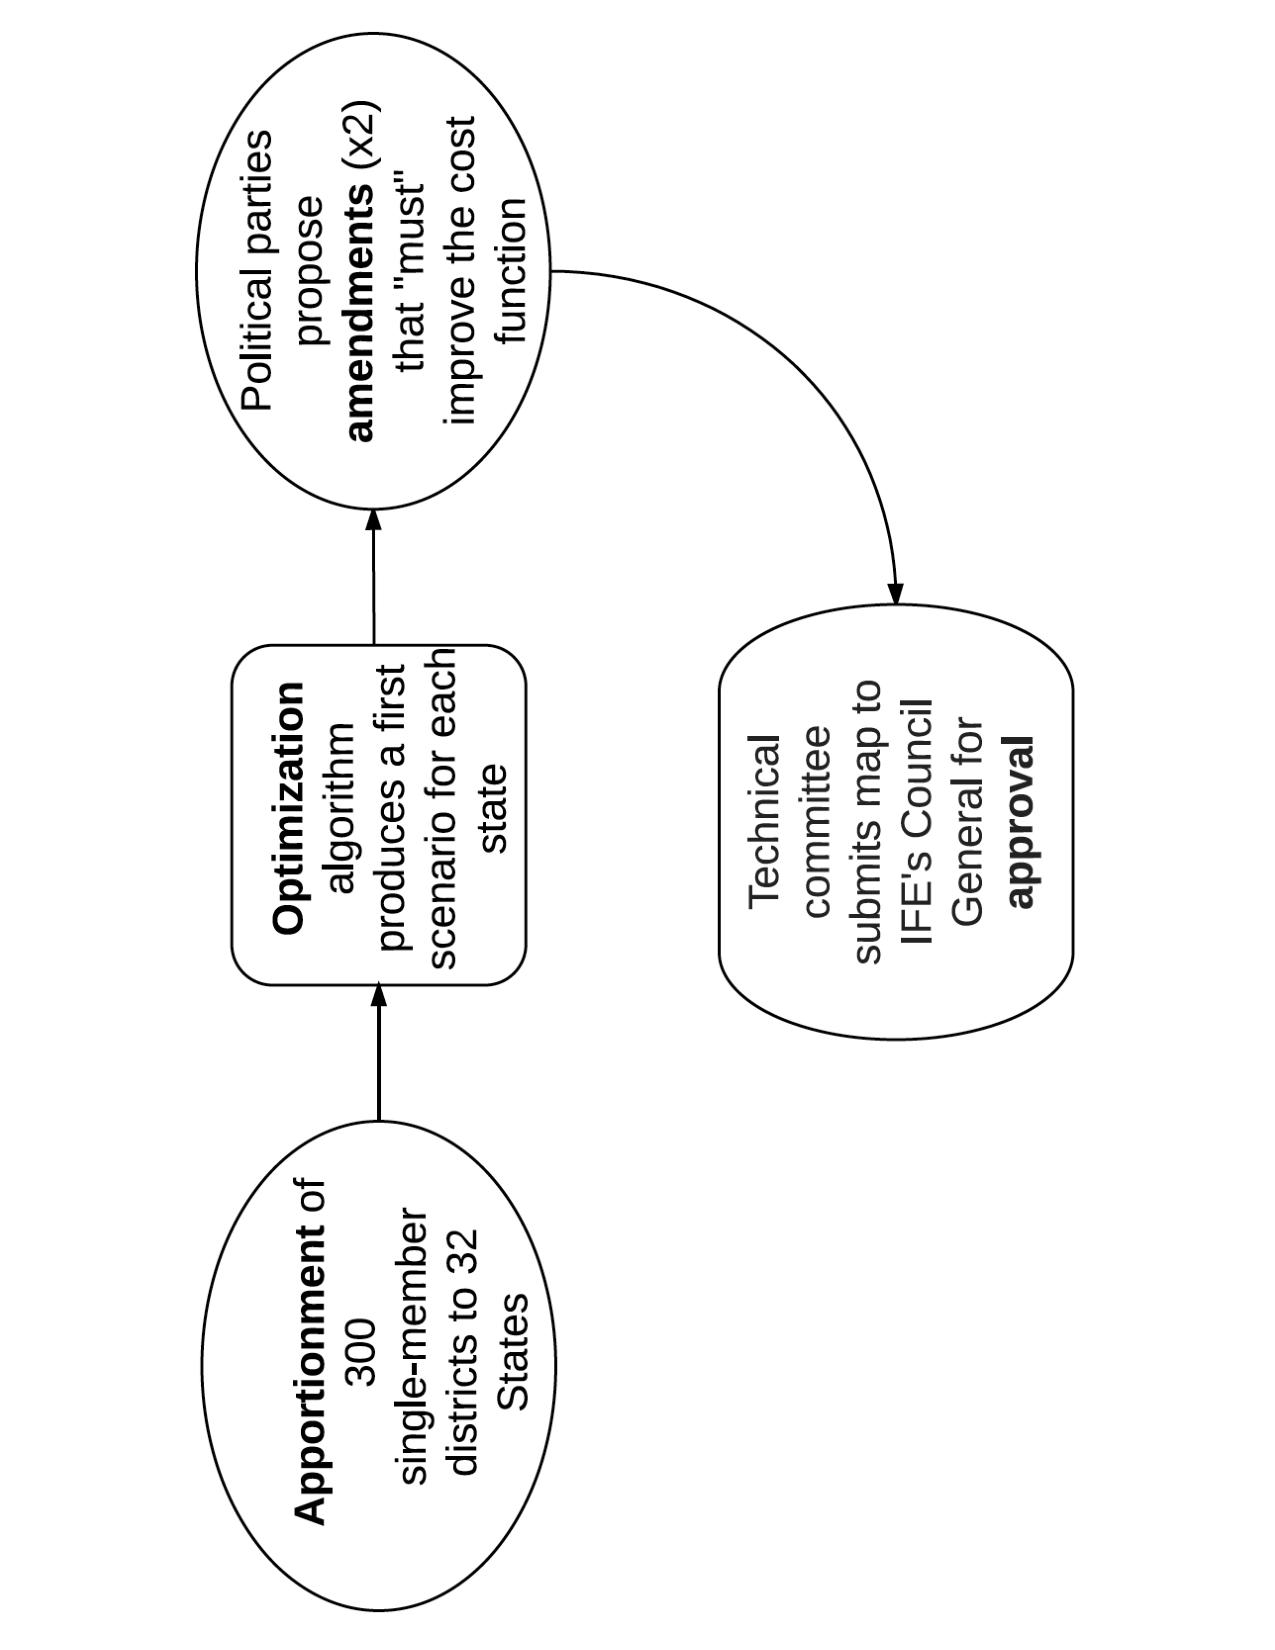
\includegraphics[width=8cm, angle=-90]{../../graphs/mexRedisProcessFlowchart.pdf}
\end{center}
}
%%%%%%%%%%%%%%%%%%%%%%%%%%%%%%%%%%%%%%%%%%%%%%%%%%%%%%%%%%%%%%%%%%%%%%%%%%%%%%%%%%%%%%%%%%%% 
\frame{                      % SLIDE
    \frametitle{The redistricting process}
% Redistricting by independent board in 1997, 2006, 2015 (abandoned, so 2018)

% \begin{enumerate}
% \item apportionment of 300 seats to 32 states
% \item optimization algorithm $\rightarrow$ proposal
% \item parties propose amendments (``must'' improve score)
% %\item repeat 2 and 3
% \item new map
% \end{enumerate}

\begin{multline*}
\texttt{Score} = .4 \times \texttt{PopBalance} + .3 \times \texttt{MunicBoundaries} \\
+ .2 \times \texttt{TravelTime} + .1 \times \texttt{Compactness}
\end{multline*}

Plus: minority representation (40\% indigenous pop.)

\bigskip

Board tolerates $\pm15\%$ imbalance to accommodate this
}
%%%%%%%%%%%%%%%%%%%%%%%%%%%%%%%%%%%%%%%%%%%%%%%%%%%%%%%%%%%%%%%%%%%%%%%%%%%%%%%%%%%%%%%%%%%% 
\frame{                      % SLIDE
    \frametitle{Optimization algorithm}
Simulated annealing = probabilistic meta-heuristic for optimization \\ locates a good approximation to the global optimum of the cost function in a large search space

\bigskip

Thousands of iterations using electoral \emph{secciones} 

\bigskip

Combinatorial optimization algorithm used to generate 
the first scenario in each state


\begin{center}
   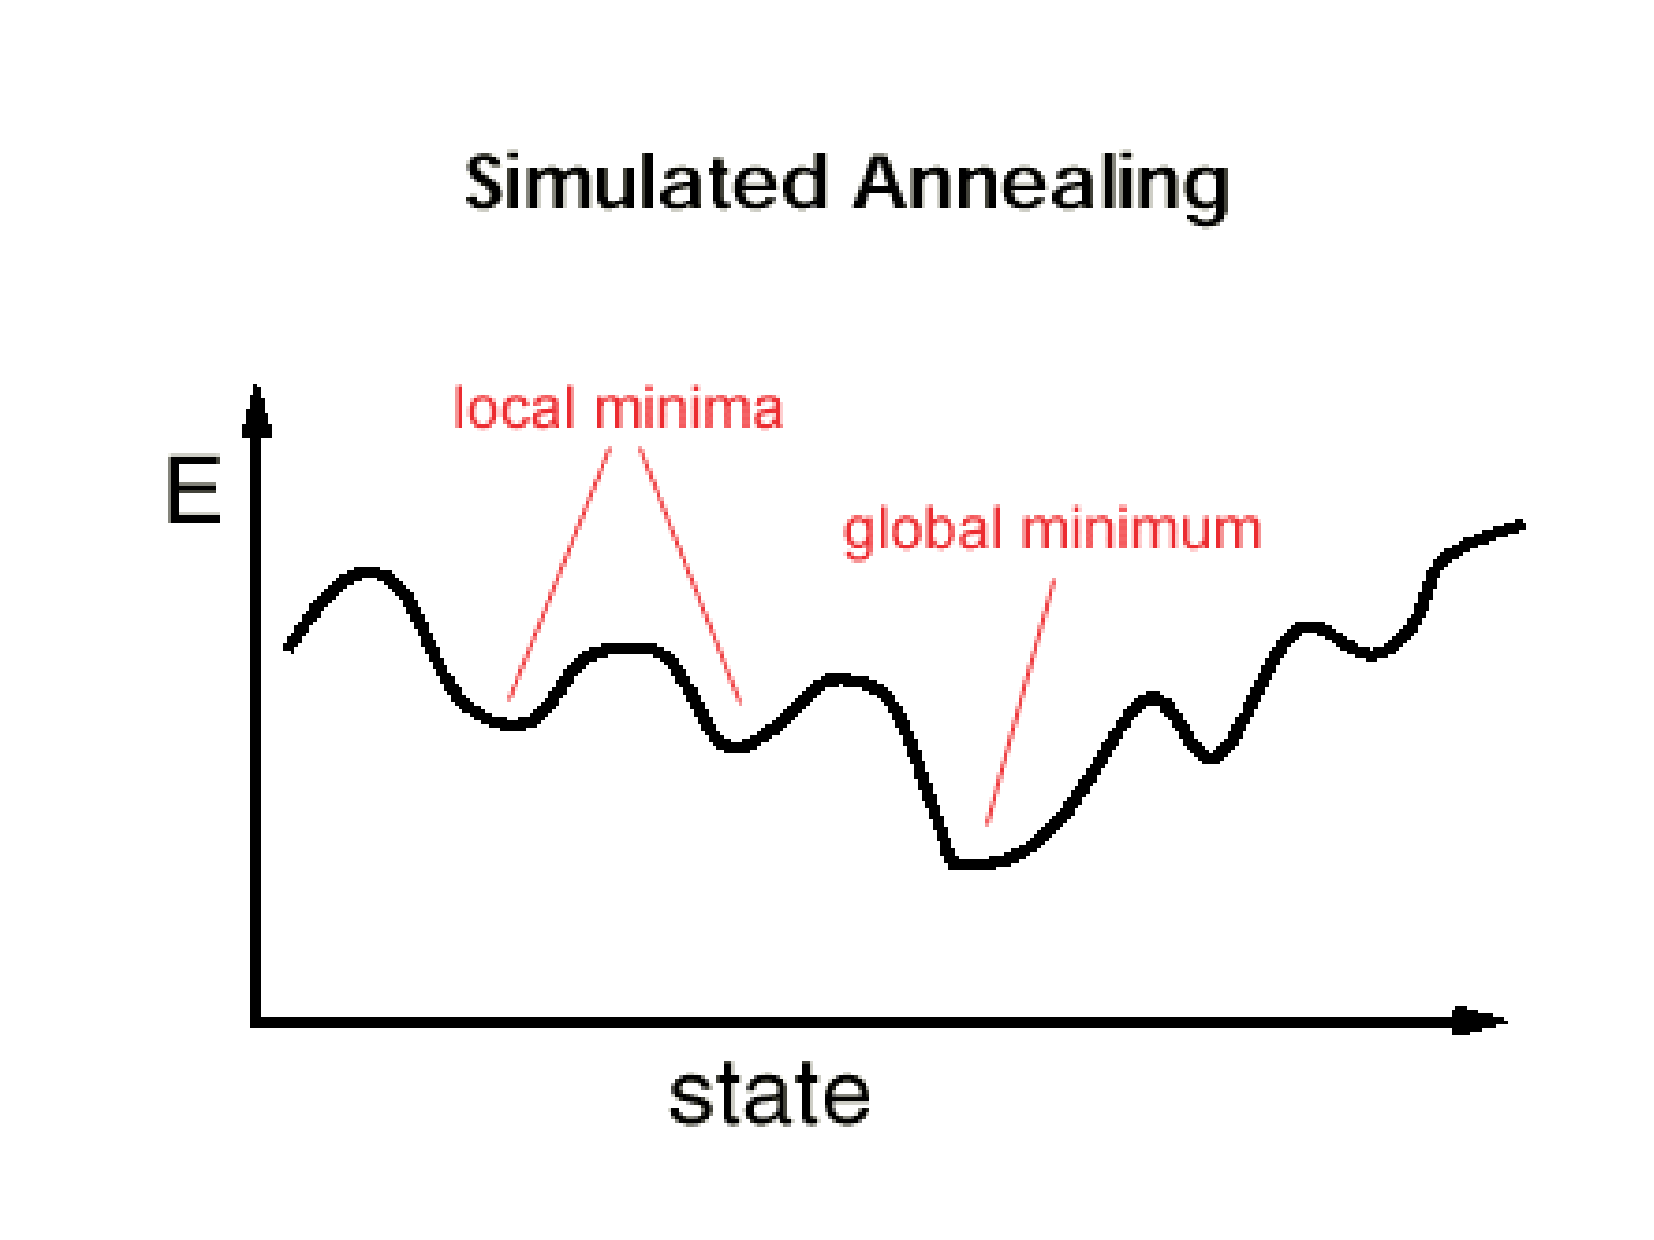
\includegraphics[width=5cm]{../../graphs/sim.pdf}
\end{center}

IFE claims that this is a public process, but the \\ operation and procedures are done \alert{behind closed doors}
}
%%%%%%%%%%%%%%%%%%%%%%%%%%%%%%%%%%%%%%%%%%%%%%%%%%%%%%%%%%%%%%%%%%%%%%%%%%%%%%%%%%%%%%%%%%%% 
\frame{                                       % SLIDE
    \frametitle{Party amendments}
\begin{center}
   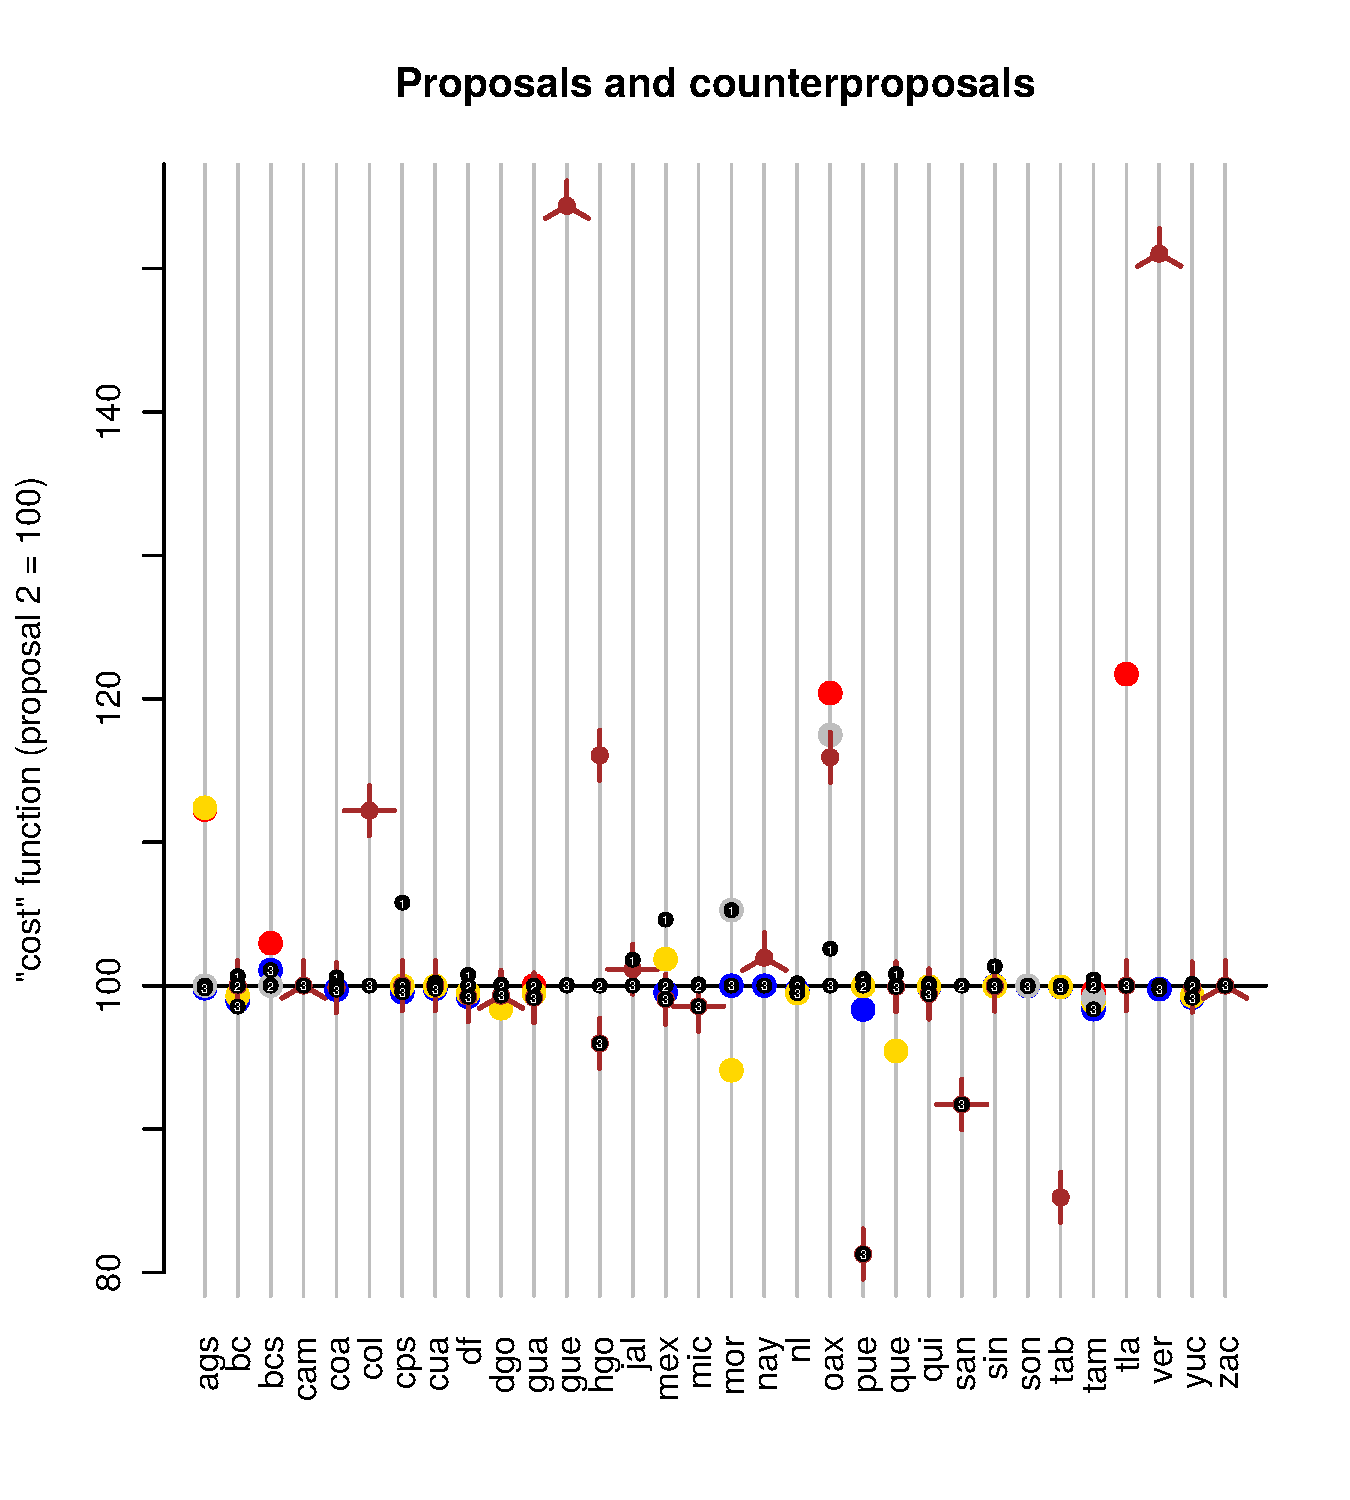
\includegraphics[width=8cm]{../../graphs/propsAndCost.pdf}
\end{center}
}
\end{document}

% %%%%%%%%%%%%%%%%%%%%%%%%%%%%%%%%%%%%%%%%%%%%%%%%%%%%%%%%%%%%%%%%%%%%%%%%%%%%%%%%%%%%%%%%%%%% 
% \frame{                                       % SLIDE
%     \frametitle{References}
% \bibliographystyle{apsrInitials}
% %\bibliography{../../bib/redMex}
% \bibliography{../../bib/magar}
% %\bibliography{/home/eric/Dropbox/mydocs/magar}
% }

